% Preamble
\documentclass[twocolumn]{aastex631}
\usepackage{natbib}
\usepackage{latexsym}
\usepackage{graphicx}
\usepackage{epsfig}
\usepackage{amssymb}
\usepackage{amsmath}
\usepackage{epstopdf}
\usepackage{hyperref}

%%%% Custom commands
\newcommand{\gradrad}{\ensuremath{\nabla_{\rm{rad}}}}
\newcommand{\gradad}{\ensuremath{\nabla_{\rm{ad}}}}
\newcommand{\justgrad}{\ensuremath{\nabla}}
\newcommand{\delp}{\ensuremath{\delta_{\rm{p}}}}
\newcommand{\Fbot}{\ensuremath{F_{\rm{bot}}}}
\newcommand{\Ftot}{\ensuremath{F_{\rm{tot}}}}
\newcommand{\Frad}{\ensuremath{F_{\rm{rad}}}}
\newcommand{\Fconv}{\ensuremath{F_{\rm{conv}}}}
\newcommand{\Fcz}{\ensuremath{F_{\rm{cz}}}}
\newcommand{\mP}{\ensuremath{\mathcal{P}}}
\newcommand{\mD}{\ensuremath{\mathcal{D}}}
\newcommand{\dP}{\ensuremath{\delta_{\rm{p}}}}
\newcommand{\Lcz}{\ensuremath{L_{\rm{CZ}}}}
\newcommand{\mR}{\ensuremath{\mathcal{R}}}
\newcommand{\mS}{\ensuremath{\mathcal{S}}}
\newcommand\Pran{\ensuremath{\mathrm{Pr}}}
\newcommand{\brunt}{Brunt-V\"{a}is\"{a}l\"{a}}

\newcommand{\angles}[1]{\langle #1 \rangle}
\newcommand{\pd}[1]{\partial_{#1}}
\renewcommand{\vec}[1]{\boldsymbol{#1}}
\newcommand{\M}[1]{\mathbf{#1}}
\renewcommand{\dot}{\vec{\cdot}}
\renewcommand{\bar}[1]{\overline{#1}}
\newcommand{\grad}{\vec{\nabla}}
\newcommand{\cross}{\vec{\times}}
\newcommand{\laplacian}{\nabla^2}

%%%% Journal preamble
\received{}
\revised{}
\accepted{}
\published{}
\submitjournal{ApJ}

\shorttitle{Convective Penetration}
\shortauthors{Anders et al}


\begin{document}

%%%% Title and Abstract
\title{Convective penetration probably parameterizes convective overshoot}
\author[0000-0002-3433-4733]{Evan H. Anders}
\affiliation{CIERA, Northwestern University, Evanston IL 60201, USA}
\author[0000-0001-5048-9973]{Adam S. Jermyn}
\affiliation{Center for Computational Astrophysics, Flatiron Institute, New York, NY 10010, USA}
\author[0000-0002-7635-9728]{Daniel Lecoanet}
\affiliation{CIERA, Northwestern University, Evanston IL 60201, USA}
\affiliation{Department of Engineering Sciences and Applied Mathematics, Northwestern University, Evanston IL 60208, USA}
\author[0000-0001-8935-219X]{Benjamin P. Brown}
\affiliation{Department Astrophysical and Planetary Sciences \& LASP, University of Colorado, Boulder, CO 80309, USA}

\correspondingauthor{Evan H. Anders}
\email{evan.anders@northwestern.edu}

\begin{abstract}
Most stars host convection zones, in which heat is transported directly by fluid motion.
Parameterizations like mixing length theory adequately describe convective flows in the bulk of these regions, but the behavior of convective boundaries is not well understood.
Here we examine how convective motions mix entropy and in turn extend the size of the convection zone, a process referred to as convective penetration.
We derive a ``penetration parameter'' $\mP$ which compares how far the radiative gradient deviates from the adiabatic gradient on either side of the Schwarzschild convective boundary.
Following \citet{roxburgh1989} and \citet{zahn1991}, we construct a model of penetration based on an energy balance, and find that the extent of penetration is controlled by $\mP$.
We perform 3D numerical simulations with Dedalus using a simplified Boussinesq model of stellar convection with a radiative flux and find good agreement with the derived theory.
We evolve these simulations for thousands of overturn times; over these long timescales our simulations consistently develop large penetrative regions.
In stellar contexts, we expect $\mathcal{P} \approx 1$ and in this regime our results suggest that convection zones may extend beyond the Schwarzschild boundary by up to $\sim$20-30\% of a mixing length.
We present a MESA solar model which employs our parameterization of convective penetration, and find that the base of the solar convection zone extends by (TODO X amount for some choice of parameters).
We further discuss prospects for extending these results to more realistic stellar contexts.
\end{abstract}
\keywords{UAT keywords}



%%%% Body of paper
\section{Introduction}
\label{sec:introduction}

\subsection{Context}
Convection is a crucial mechanism for transporting heat in stars~\citep{woosley_etal_2002, hansen_etal_2004, christensen-dalsgaard_2021}, and convective dynamics influence many poorly-understood stellar phenomena.
For example, convection drives the magnetic dynamo of the Sun, leading to a whole host of emergent phenomena collectively known as solar activity \citep{brun_browning_2017}.
Convection also mixes chemical elements in stars, which can modify observed surface abundances or inject additional fuel into their cores, thereby extending stellar lifetimes \citep{salaris_cassisi_2017}.
Furthermore, convective motions excite waves, which can be observed and used to constrain the thermodynamic structure of stars \citep{aerts2010, basu2016}.
A complete and nuanced understanding of convection is therefore crucial for understanding stellar structure and evolution, and for connecting this understand to observations.

Despite decades of study, robust parameterizations for the mechanisms broadly referred to as ``convective overshoot'' remain elusive, and improved parameterizations could resolve many discrepancies between observations and structure models.
In the stellar structure literature, ``convective overshoot'' refers to any convectively-driven mixing which occurs beyond the boundaries of the Ledoux-unstable zone.
This mixing can influence, for example, observed surface lithium abundances in the Sun and solar-type stars, which align poorly with theoretical predictions \citep{pinsonneault1997, carlos_etal_2019, dumont_etal_2021}.
Furthermore, modern spectroscopic observations suggest a lower solar metallicity than previously thought, and models computed with modern metallicity estimates and opacity tables have shallower convection zones than helioseismic observations suggest \citep{basu_antia_2004, bahcall_etal_2005, bergemann_serenelli_2014, vinyoles_etal_2017, asplund_etal_2021}; modeling and observational discrepancies can be reduced with additional mixing below the convective boundary \citep{christensen-dalsgaard_etal_2011}.

Beyond the Sun, overshooting in massive stars with convective cores must be finely tuned as a function of stellar mass, again pointing to missing physics in our current parameterizations \citep{claret_torres_2018, jermyn_etal_2018, viani_basu_2020, martinet_etal_2021, pedersen_etal_2021}.
Since core convective overshoot increases the reservoir of fuel available for nuclear fusion at each stage in stellar evolution, improved models of core convective boundary mixing could have profound impacts on the post-main sequence evolution and remnant formation of massive stars \citep{farmer_etal_2019, higgins_vink_2020}.

In order to ensure that models can be evolved on fast (human) timescales, 1D stellar evolution codes rely on simple parameterizations of convection \citep[e.g., mixing length theory,][]{bohm-vitense1958} and convective overshoot \citep{shaviv_salpeter_1973, maeder1975, herwig2000, paxton_etal_2011, paxton_etal_2013, paxton_etal_2018, paxton_etal_2019}.
While some preliminary work has been done to couple 3D dynamical convective simulations with 1D stellar evolution codes \citep{jorgensen_weiss_2019}, these calculations are prohibitively expensive to perform at every timestep in a stellar evolution simulation.
In order to resolve discrepancies between stellar evolution models and observations, a more complete and \emph{parameterizeable} understanding of convective overshoot is required.

The broad category of ``convective overshoot'' in the stellar literature is an umbrella term for a few hydrodynamical processes.
The first process is confusingly also called ``\emph{convective overshoot}'' in the fluid dynamics literature, and refers to motions which extend beyond the convective boundary but do not adjust the thermodynamic profiles.
The second process is called ``\emph{convective penetration},'' and refers to convective motions which mix the thermodynamic profiles beyond the convective boundary, thereby extending the adiabatically-mixed convective region.
We will follow a deep history \citep{zahn1991, brummell_etal_2002, korre_etal_2019} and use this terminology.
Many studies have also examined \emph{entrainment}, the process by which convection zones expand by eroding composition gradients or modifying the radiative gradient \citep[][]{meakin_arnett_2007, viallet_etal_2013, cristini_etal_2017, fuentes_cumming_2020, horst_etal_2021}.
The primary focus of this work is convective penetration.

Convective overshoot, penetration, and entrainment have been studied in the laboratory and through numerical simulations for decades, and the state of the field has been regularly reviewed \citep[e.g.,][]{marcus_etal_1983, zahn1991, browning_etal_2004, rogers_etal_2006, viallet_etal_2015, korre_etal_2019}.
Modern numerical experiments often examine the importance of the ``stiffness'' of a radiative-convective interface.
The stiffness measures the relative stability of a radiative zone and an adjacent convection zone according to some measure like a dynamical frequency or characteristic entropy gradient.
Experiments exhibiting extensive expansion of convection zones via entrainment have a long history \citep[dating back to e.g.,][and this process is often confusingly called ``penetration'']{musman1968, deardorff_etal_1969, moore_weiss_1973}.
Some recent studies in simplified Boussinesq setups exhibit stiffness-dependent convection zone expansion via entrainment \citep{couston_etal_2017, toppaladoddi_wettlaufer_2018}; others find stiffness-dependent pure overshoot \citep{korre_etal_2019}.
While a clear link between stiffness and entrainment and overshoot has seemingly emerged in these simple simulation setups, a clear mechanism for penetration remains elusive.

Studies which more closely model the conditions inside of stars have presented confusing results.
Many studies have exhibited hints of penetrative convection -- that is, mixing of the entropy gradient towards the adiabatic beyond the convective boundary \citep{hurlburt_etal_1986, hurlburt_etal_1994, singh_etal_1995, saikia_etal_2000, browning_etal_2004, rogers_etal_2006, kitiashvili_etal_2016, brun_etal_2017, pratt_etal_2017, higl_etal_2021}.
These simulations include simple plane-parallel studies of compressible convection as well as global 3D simulations which employ profiles from stellar structure codes as background states.
Unfortunately, other fundamental studies in both Cartesian and spherical geometries have exhibited little to no dependence of penetration on the stiffness \citep{brummell_etal_2002, rogers_glatzmaier_2005}.
This host of experiments suggests that convective penetration is \emph{probably} a process that happens in stars, but no clear model has emerged which explains whether convective penetration depends on stiffness or some other quantity.

There are hints in the literature that convective penetration may be dependent upon energy fluxes.
\citet{roxburgh1978, roxburgh1989, roxburgh1992, roxburgh1998} derived an ``integral constraint'' from the energy conservation equation and found that a spatial integral of the flux puts an upper limit on the size of a theoretical penetrative region.
\citet{zahn1991} theorized that convective penetration should depend only on how steeply the radiative temperature gradient varies at the convective boundary.
Following \citet{zahn1991}'s work, \citet{rempel2004} derived a semianalytic model and suggested that inconsistencies seen in simulations of penetrative dynamics can be explained by the magnitude of the fluxes or luminosities driving the simulations.
Indeed, some simulations have tested this idea, and found that penetration depths depend strongly on the input flux \citep{singh_etal_1998, kapyla_etal_2007, tian_etal_2009, hotta2017, kapyla2019}.
Furthermore, in the limit of low stiffness, the simulations of \citet{hurlburt_etal_1994} and \citet{rogers_glatzmaier_2005} may agree with Zahn's theory (although at high stiffness they disagree).
In light of these results, and the possible importance of energy fluxes, Roxburgh's integral constraint and Zahn's theory deserve to be revisited.

\subsection{Convective penetration \& this study's findings}

Convective penetration is the process by which realistic convective motions extend beyond the Schwarzschild-stable boundary and mix the entropy gradient towards the adiabatic.
\begin{quote}
\emph{
In this paper, we present simulations which exhibit convective penetration.
}
\end{quote}
This process is phenomenologically described in Sec.~\ref{sec:central_results}.

In order to understand this phenomenon, we derive theoretical predictions for the size of the penetrative zone based on the ideas of \citet{roxburgh1989} and \citet{zahn1991}.
%We design and carry out numerical experiments to test the idea that the penetration depth depends on the shape of the radiative gradient at the convective boundary.
\begin{quote}
\emph{
We find that the extent of convective penetration depends strongly on the shape and magnitude of the radiative gradient near the convective boundary.
}
\end{quote}
Thus, the penetration depth can be calculated using the radiative conductivity (or opacity) \emph{profile} near the convective boundary.

We present these findings as follows.
In Sec.~\ref{sec:central_results}, we present the central finding of this work: penetration zones in nonlinear convective simulations.
In Sec.~\ref{sec:theory}, we describe the equations used and derive a parameterized theory of convective penetration.
In Sec.~\ref{sec:simulation_details}, we describe our simulation setup and parameters.
In Sec.~\ref{sec:results}, we present the results of these simulations, with a particular focus on the depth of the penetrative regions.
In Sec.~\ref{sec:solar_model}, we create and discuss a solar MESA model which uses this theory to determine the bottom of the solar convection zone.
Finally, we discuss how future simulations can better constrain this theory in Sec.~\ref{sec:discussion}.

\begin{figure*}[t]
\centering
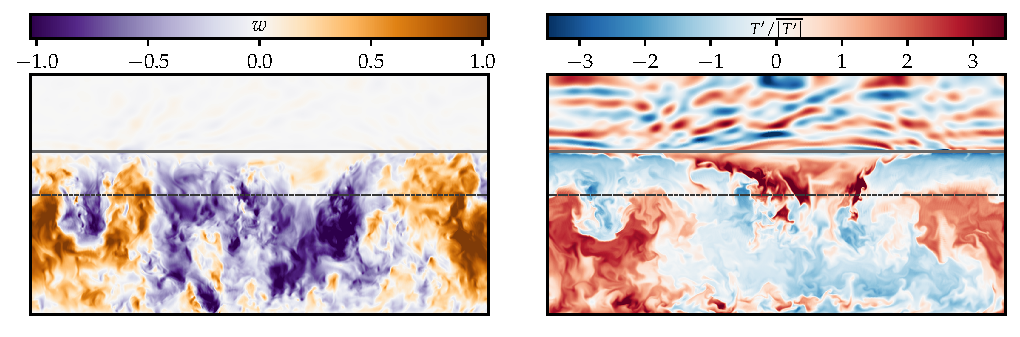
\includegraphics[width=\textwidth]{vertical_dynamics_panels.pdf}
\caption{
Displayed is an instantaneous snapshot of dynamics in a vertical slice through the simulation with $\mR = 6.4 \times 10^3$, $\mP_D = 4$ and $\mS = 10^3$ (see Sec.~\ref{sec:simulation_details}).
The Schwarzschild boundary of the convection zone where $\gradad = \gradrad$ is displayed as a dashed horizontal line.
The top of the penetrative zone ($\delta_{0.1}$, see Sec.~\ref{sec:simulation_details}) is shown by a solid horizontal line.
(Left) The vertical velocity is shown; orange convective upflows extend far past the Schwarzschild boundary of the convection zone but stop abruptly where $\justgrad$ departs from $\gradad$.
(Right) Temperature fluctuations are shown, normalized by their average magnitude at each height in order to clearly display all dynamical features.
%Unlike the vertical velocity, $T'$ shows distinctly different behavior in the CZ and PZ, switching sign at the Schwarzschild boundary of the convection zone.
\label{fig:vertical_dynamics_panels}
}
\end{figure*}

\section{Central Result: Convective Penetration}
\label{sec:central_results}

In Fig.~\ref{fig:vertical_dynamics_panels}, we display a snapshot of dynamics in an evolved simulation which exhibits convective penetration.
The simulation domain is a 3D Cartesian box, and this figure shows a vertical slice through the center of the domain.
In the left panel, we display the vertical velocity.
We see that convective motions extend beyond the Schwarzschild boundary of the convection zone, which is denoted by a horizontal dashed grey line.
These motions come to a halt at the top of a penetration zone, denoted by a solid horizontal line, where the gradient departs from the adiabatic towards the radiative gradient.
In the right panel, we display temperature perturbations away from the time-evolving mean temperature profile.
We see that warm upwellings in the Schwarzschild-unstable convection zone (below the dashed line) become cold upwellings in the penetration zone (above the dashed line), and these motions excite gravity waves in the stable radiative zone (above the solid line).

We further explore the simulation from Fig.~\ref{fig:vertical_dynamics_panels} in Fig.~\ref{fig:grad_profiles} by displaying time- and horizontally-averaged 1D profiles of the thermodynamic gradient $\justgrad$ (defined in Sec.~\ref{sec:theory}).
The adiabatic gradient $\gradad$ is shown in purple and is a constant value in the simulation.
The radiative gradient $\gradrad$ is shown in orange.
The domain exhibits a classical Schwarzshild-unstable convection zone (CZ) for $z \lesssim 1.04$ where $\gradrad > \gradad$; the upper boundary of this region is denoted by a dashed vertical line.
Above this point, $\gradrad < \gradad$ and the domain would be considered stable by the Schwarzschild criterion.
However, the evolved convective dynamics in Fig.~\ref{fig:vertical_dynamics_panels} have raised $\justgrad \rightarrow \gradad$ in an extended penetration zone (PZ) which extends from roughly $1.04 \leq z \leq 1.4$.
Above this point, $\justgrad$ departs from $\gradad$, returning to $\gradrad$ in a classical stable radiative zone (RZ).

Our goals in this paper are to understand how these PZs form, and to parameterize this effect so that it can be included in 1D stellar evolution calculations.

\newpage
\section{Theory}
\label{sec:theory}

\subsection{Equations \& flux definitions}
\label{sec:theory_equations}
Throughout this work, we will utilize a modified version of the incompressible Boussinesq equations,
\begin{align}
&\grad\dot\vec{u} = 0 
\label{eqn:incompressible} \\
&\partial_t \vec{u} + \vec{u}\dot\grad\vec{u} = -\frac{1}{\rho_0}\grad p + \frac{\rho_1}{\rho_0}\vec{g} + \nu\grad^2 \vec{u} 
\label{eqn:momentum} \\
&\partial_t T + \vec{u}\dot\grad T + w \gradad + \grad\dot[-k \grad \overline{T}] = \chi\grad^2 T' + Q
\label{eqn:temperature} \\
&\frac{\rho_1}{\rho_0} = -|\alpha| T.
\label{eqn:boussinesq}
\end{align}
Here, the density is decomposed into a constant background $\rho_0$ with fluctuations $\rho_1$ which appear only in the buoyancy force and depend on the temperature $T$ and the coefficient of thermal expansion $\alpha = \partial\ln\rho / \partial T$.
We furthermore define the velocity vector $\vec{u}$, the viscous diffusivity $\nu$, the thermal diffusivity $\chi$, the bulk internal heating $Q$, the adiabatic gradient $\gradad$, and a height-dependent thermal conductivity $k$.
We will consider Cartesian coordinates $(x, y, z)$ with a constant vertical gravity $\vec{g} = -g\hat{z}$.
Throughout this work, we will represent horizontal averages with bars ($\overline{\,\cdot\,}$) and fluctuations away from those averages with primes ($'$).
Thus, in Eqn.~\ref{eqn:temperature}, $\bar{T}$ is the horizontally averaged temperature and $T'$ are fluctuations away from that; both of these fields evolve in time according to Eqn.~\ref{eqn:temperature}.

Assuming convection reaches a time-stationary state, the fluxes are found by horizontally-averaging then vertically integrating Eqn.~\ref{eqn:temperature} to find
\begin{equation}
\overline{\Ftot} = \overline{\Frad} + \overline{\Fconv} = \int Q dz + \Fbot,
\label{eqn:flux_definition}
\end{equation}
where $\Fbot$ is the flux carried at the bottom of the domain, and $\overline{\Ftot}$ is the total flux, which can vary in height due to the heating $Q$.
We allow the mean temperature profile $\overline{T}$ to carry a radiative flux $\bar{\Frad} = -k \grad \overline{T}$.
We note that $k$ and $-\partial_z \bar{T}$ fully specify $\bar{\Frad}$ and in turn the convective flux, $\bar{\Fconv} = \bar{\Ftot} - \bar{\Frad}$.
We define the gradient and radiative gradient 
\begin{equation}
\justgrad \equiv -\partial_z \bar{T} \qquad
\gradrad \equiv \frac{\bar{\Ftot}}{k}.
\label{eqn:gradrad_definition}
\end{equation}
We have defined the $\justgrad$'s as positive quantities to align with stellar structure conventions and intuition.
Marginal stability is achieved when $\justgrad = \gradad$, a constant.
We note that the classical Schwarzschild boundary of the convection zone is the height $z = L_s$ at which $\gradrad = \gradad$ and $\bar{\Fconv} = 0$.

The addition of a nonzero $\gradad$ to Eqn.~\ref{eqn:temperature} was derived by \citet{spiegel_veronis_1960} and utilized by e.g., \citet{korre_etal_2019}.
In this work, we have decomposed the radiative diffusivity into a background portion ($\grad\dot \bar{\Frad}$) and a fluctuating portion ($\chi \grad^2 T'$); by doing so, we have introduced a height-dependent $\gradrad$ to the equation set while preserving the diffusive behavior on fluctuations felt by classical Rayleigh-B\'{e}nard convection.
Here, we will assume a model in which an unstable convection zone ($\gradrad > \gradad$) sits below a stable radiative zone ($\gradrad < \gradad$), but the same logic applies to the inverted problem.

\subsection{Kinetic energy \& the dissipation-flux link}
\label{sec:theory_energy}

\begin{figure}[t]
\centering
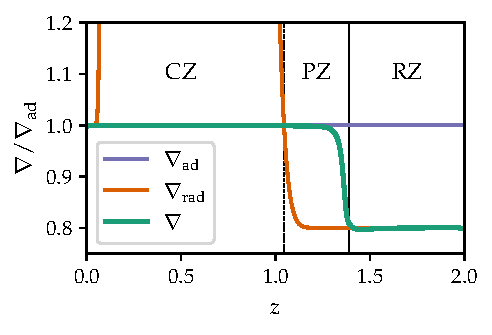
\includegraphics[width=\columnwidth]{grad_profiles.pdf}
\caption{
Measured time- and horizontally-averaged vertical profiles of the thermodynamic gradients from the simulation in Fig.~\ref{fig:vertical_dynamics_panels}.
We plot $\justgrad$ (green) compared to $\gradad$ (purple, a constant) and $\gradrad$ (orange); note the extended penetration zone (PZ) where $\justgrad \approx \gradad > \gradrad$.
\label{fig:grad_profiles}
}
\end{figure}


Taking a dot product of the velocity and Eqn.~\ref{eqn:momentum} reveals the kinetic energy equation,
\begin{equation}
\frac{\partial \mathcal{K}}{\partial t}
+ \grad\dot\mathcal{F}
= \mathcal{B} - \Phi,
%\frac{\partial}{\partial t}\left(\frac{|\vec{u}|^2}{2}\right) 
%+ \grad\dot\left[\vec{u}\left(\frac{|\vec{u}|^2}{2} + \frac{p}{\rho_0}\right) - \nu\vec{u}\cross\vec{\omega}\right]
%= |\alpha| g w T - \nu|\vec{\omega}|^2,
\label{eqn:kinetic_energy}
\end{equation}
where we define the kinetic energy $\mathcal{K} \equiv |\vec{u}|^2/2$, the fluxes of kinetic energy $\mathcal{F} \equiv \left[\vec{u}(\mathcal{K} + p/\rho_0) - \nu\vec{u}\cross\vec{\omega} \right]$, the buoyant energy generation rate $\mathcal{B} \equiv |\alpha| g w T'$, and the viscous dissipation rate $\Phi \equiv \nu |\vec{\omega}|^2$ where $\vec{\omega} = \grad\cross\vec{u}$ is the vorticity and $|\vec{u}|^2 = \vec{u}\dot\vec{u}$ \& $|\vec{\omega}|^2 = \vec{\omega}\dot\vec{\omega}$.
We next take a horizontal- and time-average of Eqn.~\ref{eqn:kinetic_energy} (we absorb the time-average into the horizontal-average $\bar{\,\cdot\,}$ notation for simplicity).
Assuming that $\bar{\mathcal{K}}$ reaches a statistically stationary state, convective motions satisfy
\begin{equation}
\frac{d\bar{\mathcal{F}}}{dz} = \bar{\mathcal{B}} - \bar{\Phi}.
\label{eqn:kinetic_energy_1D}
\end{equation}
It is reasonable to assume that $\mathcal{F}$ is zero at the boundaries of the convecting region (see Fig.~\ref{fig:theory_profiles}, upper panel).
We integrate Eqn.~\ref{eqn:kinetic_energy_1D} vertically between these zeros of the flux to find
\begin{equation}
\int \bar{\mathcal{B}}\,dz = \int \bar{\Phi}\,dz.
\label{eqn:integral_constraint}
\end{equation}
Integral constraints of this form are the basis for a broad range of analyses in Boussinesq convection \citep[see e.g.,][]{ahlers_etal_2009, goluskin2016} and were considered in the context of penetrative stellar convection by \citet{roxburgh1989}.
Eqn.~\ref{eqn:integral_constraint} is the straightforward statement that work by buoyancy on large scales must be balanced by viscous dissipation on small scales.

\begin{figure}[t!]
\centering
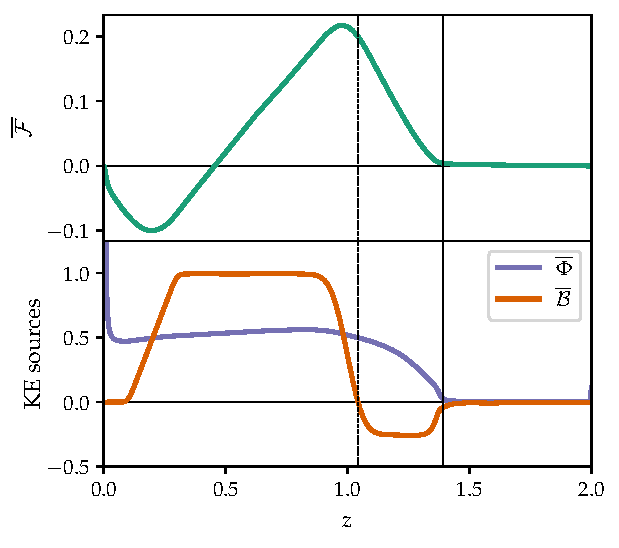
\includegraphics[width=\columnwidth]{theory_profiles.pdf}
\caption{
(upper) The vertical profile of the horizontally-averaged kinetic energy fluxes $\bar{\mathcal{F}}$ realized in the simulation shown in Fig.~\ref{fig:vertical_dynamics_panels}. 
$\bar{\mathcal{F}}$ is zero at the bottom boundary, the top of the penetrative region (marked by a solid line) and again at the mid-convection zone (marked by a dashed line).
Eqn.~\ref{eqn:integral_constraint} must hold true over an integral between any two of these zeros.
Here, we have neglected the viscous portion of the fluxes; this contributes negligibly in the bulk, and is zero by construction at $z = [0, 2]$.
(bottom) Source terms from Eqn.~\ref{eqn:kinetic_energy_1D} normalized by the maximum of $\overline{\mathcal{B}}$ ($\bar{\mathcal{F}}$ in the left panel is normalized in the same manner).
\label{fig:theory_profiles}
}
\end{figure}



We now find it instructive to break up the convecting region into a Schwarzschild-unstable ``convection zone'' (CZ) and a extended ``penetration zone'' (PZ); we assume that convective motions efficiently mix $\justgrad \rightarrow \gradad$ in both the CZ and PZ.
We note that the buoyant energy generation is proportional to the convective flux, $\bar{\mathcal{B}} = |\alpha|g\bar{w T'} = |\alpha| g \bar{\Fconv}$.
Thus, in the PZ where $\gradad > \gradrad$ (see Fig.~\ref{fig:theory_profiles}, middle panel), we know that $\bar{\Fconv} < 0$ and so $\bar{\mathcal{B}} < 0$ too (see the discussion around Eqn.~\ref{eqn:gradrad_definition}).
Breaking up Eqn.~\ref{eqn:integral_constraint}, we see that
\begin{equation}
%\int_{\rm{CZ}} \bar{\mathcal{B}}\,dz \qquad=\qquad
\int_{\rm{CZ}} \bar{\mathcal{B}}\,dz \,\,=\,\,
\int_{\rm{CZ}} \bar{\Phi}\,dz + \int_{\rm{PZ}} \bar{\Phi}\,dz + \int_{\rm{PZ}}(-\bar{\mathcal{B}})\,dz.
\label{eqn:constraint_cz_pz_split}
\end{equation}
Eqn.~\ref{eqn:constraint_cz_pz_split} is thus arranged so that the (positive) buoyant engine of convection is on the left-hand side, and the (positive) sinks of work are on the RHS.
We see that the size of the PZ is set by some combination of viscous dissipation and buoyancy breaking.
We now parameterize the fraction of the buoyant engine consumed by CZ dissipation  
\begin{equation}
f \equiv \frac{\int_{\rm{CZ}} \bar{\Phi}\,dz}{\int_{\rm{CZ}}\bar{\mathcal{B}}\,dz}.
\label{eqn:f_defn}
\end{equation}
Under this parameterization, Eqn.~\ref{eqn:constraint_cz_pz_split} can be written
\begin{equation}
\frac{\int_{\rm{PZ}}(-\bar{\mathcal{B}})\,dz}{\int_{\rm{CZ}} \bar{\mathcal{B}}\,dz}
+ \frac{\int_{\rm{PZ}} \bar{\Phi}\,dz }{\int_{\rm{CZ}} \bar{\mathcal{B}}\,dz}
= (1 - f),
\label{eqn:first_pz_parameterization}
\end{equation}
and we can immediately read off limits on a hypothetical PZ according to $f$,
\begin{enumerate}
\item Viscous dissipation is inefficient in the limit that $f \rightarrow 0$.
Reasonably also assuming that $\int_{\rm{PZ}}\bar{\Phi}\,dz \rightarrow 0$, Eqn.~\ref{eqn:first_pz_parameterization} states that the PZ must be large enough for its negative buoyant work to be equal in magnitude to the positive buoyant work of the CZ.
This is the integral constraint on the maximum size of the PZ that \citet{roxburgh1989} derived.
\item In the limit that $f \rightarrow 1$, viscous dissipation efficiently counteracts the buoyancy work in the CZ.
Per Eqn.~\ref{eqn:first_pz_parameterization}, the positive-definite PZ terms must approach zero and no PZ develops in this limit.
This is mathematically equivalent to standard boundary-driven convection experiments.
\end{enumerate}
In general, we anticipate from the results of e.g., \citet{currie_browning_2017} that $f$ is closer to 1 than 0, but its precise value must be measured directly from simulations.
Indeed, we find that $f \gg 0$ but $f < 1$ in our simulations (see e.g., Fig.~\ref{fig:theory_profiles}, bottom panel\footnote{the bulk dynamics suggest by eye $f \sim 0.5$, but due to e.g., the height dependence of $\bar{\mathcal{B}}$ in our simulations we measure $f \approx 0.74$.}).

Assuming that a PZ of depth $\delp$ develops above a CZ of depth $L_{\rm{CZ}}$, we model the PZ dissipation as
\begin{equation}
\int_{\rm{PZ}} \bar{\Phi}\,dz = \xi\frac{\delp}{L_{\rm{CZ}}}\int_{\rm{CZ}}\bar{\Phi}\,dz = \xi \delp \Phi_{\rm{CZ}}.
\label{eqn:xi_defn}
\end{equation}
Here $\Phi_{\rm{CZ}}$ is the volume-averaged dissipation value in the CZ and $\xi$ is a measurable parameter bounded by ${[0, 1]}$ that describes the shape of the dissipation profile as a function of height in the PZ.
In words, we assume that $\bar{\Phi}(z = L_s) \approx \Phi_{\rm{CZ}}$ at the CZ-PZ boundary and that $\bar{\Phi}$ decreases with height in the PZ.
The shape of $\bar{\Phi}$ determines $\xi$; a linear falloff gives $\xi = 1/2$, a quadratic falloff gives $\xi = 2/3$, and $\xi = 1$ assumes no falloff.
With this parameterization, and $\bar{\mathcal{B}} \propto \bar{\Fconv}$, we rewrite Eqn.~\ref{eqn:first_pz_parameterization}
\begin{equation}
-\frac{\int_{\rm{PZ}}\bar{\Fconv}\,dz}{\int_{\rm{CZ}}\bar{\Fconv}\,dz} + f\xi\frac{\delp}{L_{\rm{CZ}}}
= (1 - f).
\label{eqn:theory_fraction}
\end{equation}
In order to derive a specific prediction for the PZ depth, one must specify the vertical shape of $\overline{\Fconv}$.
We will study two cases in this work, laid out below.
In both of these cases, we define a nondimensional ``Penetration Parameter'' whose magnitude is set by the ratio of the convective flux some equidistant length $\epsilon$ above and below the Schwarzschild convective boundary $L_s$ (assuming $\justgrad = \gradad$ in the CZ and PZ),
\begin{equation}
\mP \equiv -\frac{\overline{\Fconv}(z = L_s - \epsilon)}{\overline{\Fconv}(z = L_s + \epsilon)}
= -\frac{\bar{\Fconv}_{\rm{CZ}}}{\bar{\Fconv}_{\rm{PZ}}}.
\label{eqn:theory_P_defn}
\end{equation}
Since $\Fconv < 0$ in the PZ, the sign of $\mP$ is positive.
Intuitively, $\mP$ describes which terms are important in Eqn.~\ref{eqn:first_pz_parameterization}.
When $\mP \ll 1$, the buoyancy term dominates in the PZ and dissipation can be neglected there.
When $\mP \gg 1$, buoyancy is negligible and dissipation constrains the size of the PZ.
When $\mP \sim 1$, both terms matter.

The fundamental result of this theory is Eqn.~\ref{eqn:theory_fraction}, which is a parameterized and generalized form of \citet{roxburgh1989}'s integral constraint.
This equation is also reminiscent of \citet{zahn1991}'s theory, and says that the size of a PZ is set by the profile of $\gradrad$ near the convective boundary (which we quantify in Eqn.~\ref{eqn:theory_P_defn}).
The parameters $f$ and $\xi$ are measurables which can be constrained by direct numerical simulations.
In general, we expect that $f$ and $\xi$ should not change too drastically with other simulation parameters.



\subsubsection{Case I: Discontinuous flux}
\label{sec:discontinuous_theory}
We first consider a model which satisfies
\begin{equation}
\overline{\Fconv}(z) = \Fcz \begin{cases}
1			&	z \leq L_s,\\
-\mP_D^{-1}  & 	z > L_s 
\end{cases}.
\end{equation}
Here, $\Fcz$ is a constant value of flux carried in the convection zone and $\mP_D$ is the penetration parameter (subscript D for discontinuous case).
Plugging this functional form of the flux into Eqn.~\ref{eqn:theory_fraction}, and integrating the CZ over a depth $L_{\rm{CZ}}$ below $L_s$ and the PZ over a depth $\delp$ above $L_s$, we predict
\begin{equation}
\frac{\delp}{\Lcz} = \mP_D \frac{1 - f}{1 + \xi f \mP_D}.
\label{eqn:discontinuous_prediction}
\end{equation}
Assuming that $f$ is a weak function of $\mP_D$, we see that the size of the penetration region is roughly linearly proportional to $\mP_D$, but saturates as $\mP_D \rightarrow \infty$ due to dissipation at large $\mP_D$.
Intuitively, this result makes sense: as $\mP_D$ grows, the magnitude of $\overline{\Fconv}$ and the breaking force of buoyancy in the PZ shrink, resulting in larger penetrative regions (but this growth cannot extend indefinitely).

\subsubsection{Case II: Piecewise linear flux}
\label{sec:linear_theory}
We next assume that $\overline{\Fconv}(z)$ is not discontinuous at the CZ-PZ boundary, but that its derivative may be,
\begin{equation}
\overline{\Fconv}(z) = 
\frac{\partial \Frad}{\partial z}\bigg|_{\rm{CZ}}
\begin{cases}
(L_s - z) & z \leq L_s \\
-\mP_L^{-1} (z - L_s) & z > L_s
\end{cases},
\end{equation}
where $(\partial \Frad / \partial z)|_{\rm{CZ}}$ is a constant and $\mP_L$ is the penetration parameter (subscript L for linear case).
When $\mP_L = 1$, $\bar{\Fconv}$ is just a linear profile that crosses through zero at $z = L_s$.
Again, solving Eqn.~\ref{eqn:theory_fraction} with this functional form of the flux and integrating over $L_{\rm{CZ}}$ in the CZ and $\delp$ in the PZ, we retrieve a quadratic equation.
This equation has two solution branches, only one of which corresponds to a positive value of $\delp$.
On that branch, we find
\begin{equation}
\frac{\delp}{\Lcz} = \sqrt{\mP_L (1 - f)} \,\,(\sqrt{\zeta^2 + 1} - \zeta),
\label{eqn:linear_prediction}
\end{equation}
where $\zeta \equiv (\xi f/2)\sqrt{\mP_L/(1-f)}$.
So we expect the penetration depth to be roughly proportional to $\sqrt{\mP_L}$ for small values of $\mP_L$, and to again saturate at large values of $\mP_L$. 

In this work, we will test the predictions of Eqns.~\ref{eqn:discontinuous_prediction} and \ref{eqn:linear_prediction}.
Our goals are to see if the predicted scalings with the penetration parameter $\mP$ are realized in simulations, and to measure the values of $f$ and $\xi$.

\section{Simulation Details}
We nondimensionalize Eqns.~\ref{eqn:incompressible}-\ref{eqn:boussinesq} on the length scale of the Schwarzschild-unstable convection zone $L_s$, the timescale of freefall across that convection zone $\tau_{\rm{ff}}$, and the temperature scale of the internal heating over that freefall time $\Delta T$,
\begin{equation}
\begin{split}
&T^* = (\Delta T)T = Q_0 \tau_{\rm{ff}} T,\qquad
Q^* = Q_0 Q,
\\
&\partial_{t^*} = \tau_{\rm{ff}}^{-1}\partial_t = \left(\frac{|\alpha| g Q_0}{L_s}\right)^{1/3} \partial_t,\,\,\,\,\,
\grad^* = L_s^{-1} \grad,
\\
&\vec{u}^* = u_{\rm{ff}}\vec{u} = \left(|\alpha| g Q_0 L_s^2\right)^{1/3}\vec{u},\qquad
p^* = \rho_0 u_{\rm{ff}}^2\varpi,
\\
&k^* = (L_s^2 \tau_{\rm{ff}}^{-1})k,\qquad
\mR = \frac{u_{\rm{ff}} L_s}{\nu},\qquad
\Pran = \frac{\nu}{\chi}.
\end{split}
\end{equation}
For convenience, here we define quantities with $*$ (e.g., $T^*$) as being the ``dimensionful'' quantities of Eqns.~\ref{eqn:incompressible}-\ref{eqn:boussinesq}.
Henceforth, quantities without $*$ (e.g., $T$) are dimensionless.
The dimensionless equations of motion are
\label{sec:simulation_details}
\begin{align}
&\grad\dot\vec{u} = 0 
\label{eqn:nondim_incompressible} \\
&\partial_t \vec{u} + \vec{u}\dot\grad\vec{u} = -\grad \varpi + T \hat{z} + \mR^{-1}\grad^2 \vec{u}
\label{eqn:nondim_momentum} \\
\begin{split}
\partial_t T + \vec{u}\dot\grad T + w \grad_{\rm{ad}}  + \grad\dot[-k \grad \overline{T}]\qquad\qquad 
\\
\qquad\qquad\qquad\qquad\qquad= (\Pran\mR)^{-1}\grad^2 T' + Q.
\label{eqn:nondim_temperature}
\end{split}
\end{align}
We construct a domain in the range $z \in [0, L_z]$ and choose $L_z \geq 2$ so that the domain is at least twice as deep as the Schwarzschild-unstable convection zone.
We decompose the temperature field into a time-stationary initial background profile and fluctuations, $T(x, y, z, t) = T_0(z) + T_1(x, y, z, t)$.
$T_0$ is constructed with $\justgrad = \gradad$ for $z \leq L_s$, and $\justgrad = \gradrad$ above $z > L_s$.
We impose a fixed-flux boundary at the bottom of the box ($\partial_z T_1 = 0$ at $z = 0$) and a fixed temperature boundary at the top of the domain ($T_1 = 0$ at $z = L_z$).
We generally impose impenetrable, no-slip boundary conditions at the top and bottom of the box so that $\vec{u} = 0$ at $z = [0, L_z]$.
For a select few simulations, we impose stress-free instead of no-slip boundary conditions ($w = 0$ and $\partial_z u = \partial_z v = 0$ at $z = [0, L_z]$).

We impose a constant internal heating which spans only part of the convection zone,
\begin{equation}
Q = \begin{cases}
0		& z < 0.1\,\,\rm{or}\,\,z\geq 0.1 + \delta_H,\\
Q_{\rm{mag}}		& 0.1 \leq z \leq 0.1 + \delta_H
\end{cases}.
\label{eqn:sim_Q}
\end{equation}
The integrated value of the flux through the system from the heating is therefore $F_H = \int_0^{L_z} Q_{\rm{mag}} dz = Q_{\rm{mag}}\delta_H$.
Throughout this work we choose $Q_{\rm{mag}} = 1$ and $\delta_H = 0.2$ so $F_H = 0.2$.
We offset this heating from the bottom boundary to $z = 0.1$ to avoid heating within the bottom impenetrable boundary layer where velocities go to zero and $k$ is small; this prevents strong temperature gradients from establishing there.
Furthermore, since the conductivity is not zero at the bottom boundary, the adiabatic temperature gradient there carries some flux, $\Fbot = \mu F_H$ and we choose $\mu = 10^{-3}$ so that most of the flux in the convection zone is carried by the convection.

We expect the average convective velocities to depend on the magnitude of the heating, $\angles{\vec{|u|}} \approx Q_{\rm{mag}}^{1/3} \approx 1$, so the characteristic convective frequency is $f_{\rm{conv}} \approx \angles{\vec{|u|}} / L_s \approx 1$.
The stiffness is defined,
\begin{equation}
\mS \equiv \frac{N^2}{f_{\rm{conv}}^2} \approx N^2,
\end{equation}
where $N^2$ is the \brunt$\,$frequency in the radiative zone.
In our nondimensionalization, $N^2 = \gradad - \gradrad$.
We treat $\mS$ as a control parameter; by choosing a value of the stiffness we set the magnitude of $\justgrad$, which in turn sets the value of $k$ in the radiative zone.

The crucial place in which our model differs from that of prior work is that we define the ``Penetration Parameter,'' $\mP$, according to Eqn.~\ref{eqn:theory_P_defn}.
We construct our experiments so that $\mP$ and $\mS$ can be varied separately.
We suspect that some past experiments have implicitly set $\mP \approx \mS^{-1}$, which would result in negligible penetration for high stiffness.
However, more fundamentally (as we will show in Sec.~\ref{sec:results}), the development of penetrative zones is a slow process and it is possible that many prior studies did not evolve simulations for long enough to see these regions saturate.

Aside from $\mS$ and $\mP$, the two remaining control parameters $\mR$ and $\Pran$ determine the degree of turbulence.
The value of $\mR$ roughly corresponds to the value of the peak Reynolds number $\rm{Re} = \mR |\vec{u}|$ measured in the simulations, and we set the ratio of the diffusivities $\Pran = 0.5$ throughout this work.
Astrophysical convection is in the limit of $\Pran \ll 1$ \citep{garaud2021}; we choose a modest value of $\Pran$ which slightly separates the scales between thermal and viscous structures while still allowing us to achieve convection with large Reynolds and P\'{e}clet numbers.

\subsection{Case I: Discontinuous flux}
Most of the simulations in this paper have a discontinuous convective flux at the Schwarzschild convective boundary.
We achieve this by constructing a discontinuous radiative conductivity,
\begin{equation}
k = \begin{cases}
k_{\rm{CZ}}	&	z < 1 \\
k_{\rm{RZ}} &	z \geq 1
\end{cases},
\label{eqn:sim_discontinuous_k}
\end{equation}
where CZ refers to the convection zone and RZ refers to the radiative zone (some of which will be occupied by the penetrative zone PZ).
Leaving $\mS$ and $\mP_D$ as free parameters and requiring that $\gradad$ carries $\Fbot$ at $z = 0$ and that $\gradrad$ carries $F_H + \Fbot$ for $z \geq 1$ specifies this system fully,
\begin{equation}
\begin{split}
&k_{\rm{RZ}} = \frac{\delta_H}{\mS\mP_D},\\
&k_{\rm{CZ}} = k_{\rm{RZ}}\frac{1}{1 + \mu + \mP_D^{-1}},\\
&\gradad = Q_{\rm{mag}}\mS\mP_D(1 + \mu + \mP_D^{-1}),\\
&\gradrad = \gradad - Q_{\rm{mag}}\mS.
\end{split}
\end{equation}

We study three sweeps through the ($\mP_D$, $\mS$, $\mR$) parameter space in this paper in which we hold two of these parameters constant and vary the other.
We study an additional sweep through $\mR$ parameter space using stress-free boundaries to compare to our no-slip cases.
%We use reference values of $\mP_D = 4$, $\mS = 10^3$, and $\mR = 400$; all parameter space sweeps pass through these values.
According to Eqn.~\ref{eqn:discontinuous_prediction}, we expect $\delp \propto \mP_D$.

\subsection{Case II: Piecewise linear flux}
We additionally study a select few simulations where the flux's gradient may be discontinuous at the Schwarzschild convective boundary.
We achieve this by constructing a radiative conductivity with a piecewise discontinuous gradient,
\begin{equation}
\partial_z k = \partial_z k_0
\begin{cases}
1	&	z < 1 \\
\mP_L^{-1} &	z \geq 1
\end{cases}
\label{eqn:sim_linear_k}
\end{equation}
Since $k$ varies with height, the value of $\mS$ and $\mP$ also vary with height; we specify their values at $z = 2$.
By this choice, we require
\begin{equation}
\partial_z k_0 = \frac{\delta_H}{L_s \mS \psi},\qquad
k_b = \frac{\delta_H\mu}{\mS\psi},\qquad
\gradad = Q \mS \psi,
\end{equation}
where $\psi \equiv 1 + \mP_L(1 + \mu)$.
%In these simulations, we hold $\mS = 10^3$ and $\mR = 800$ while varying $\mP_L$.
We will study one sweep through $\mP_L$ space at fixed $\mR$ and $\mS$.
According to Eqn.~\ref{eqn:linear_prediction}, we expect $\delta_p \propto \mP_L^{1/2}$.

\subsection{Numerics}
\label{sct:numerics}
We time-evolve equations \ref{eqn:nondim_incompressible}-\ref{eqn:nondim_temperature} using the Dedalus pseudospectral solver \citep{burns_etal_2020}\footnote{we use commit \href{https://github.com/DedalusProject/dedalus/commit/efb13bdaa09816dde3eee897bc2a15fc284ea2f1}{efb13bd}; the closest stable release to this commit is \href{https://github.com/DedalusProject/dedalus/releases/tag/v2.2006}{v2.2006}.} using timestepper SBDF2 \citep{wang&ruuth2008} and safety factor 0.35.
All fields are represented as spectral expansions of $n_z$ Chebyshev coefficients in the vertical ($z$) direction and as ($n_x$,$n_y$) Fourier coefficients in the horizontal ($x$,$y$) directions; our domains are therefore horizontally periodic.
We use a domain aspect ratio of two so that $x \in [0, L_x]$ and $y \in [0, L_y]$ with $L_x = L_y = 2 L_z$.
To avoid aliasing errors, we use the 3/2-dealiasing rule in all directions.
To start our simulations, we add random noise temperature perturbations with a magnitude of $10^{-3}$ to a background temperature profile $\overline{T}$; we discuss the choice of $\overline{T}$ in appendix \ref{app:accelerated_evolution}.
In some simulations we start with $\bar{T} = T_0$, described above, and in others we impose an established penetrative zone in the initial state $\bar{T}$ according to Eqn.~\ref{eqn:initial_grad}.

Spectral methods with finite coefficient expansions cannot capture true discontinuities.
In order to approximate discontinuous functions such as Eqns.~\ref{eqn:sim_Q}, \ref{eqn:sim_discontinuous_k}, and \ref{eqn:sim_linear_k}, we must use smooth transitions.
To create these smooth transitions, we define an approximate Heaviside step function using the error function,
\begin{equation}
H(z; z_0, d_w) = \frac{1}{2}\left(1 + \mathrm{erf}\left[\frac{z - z_0}{d_w}\right]\right).
\label{eqn:heaviside}
\end{equation}
In the limit that $d_w \rightarrow 0$, this function behaves identically to the classical Heaviside function centered at $z_0$.
While constructing Eqn.~\ref{eqn:sim_Q} and Eqn.~\ref{eqn:sim_linear_k}, we use $d_w = 0.02$; while constructing Eqn.~\ref{eqn:sim_discontinuous_k} we use $d_w = 0.075$.
In all other cases, we use $d_w = 0.05$.

A table describing all of the simulations presented in this work can be found in Appendix~\ref{app:simulation_table}.
We produce the figures in this paper using matplotlib \citep{hunter2007, mpl3.3.4}.
All of the Python scripts used to run the simulations in this paper and to create the figures in this paper are publicly available in a git repository, found at [CITE].

\begin{figure*}[t]
\centering
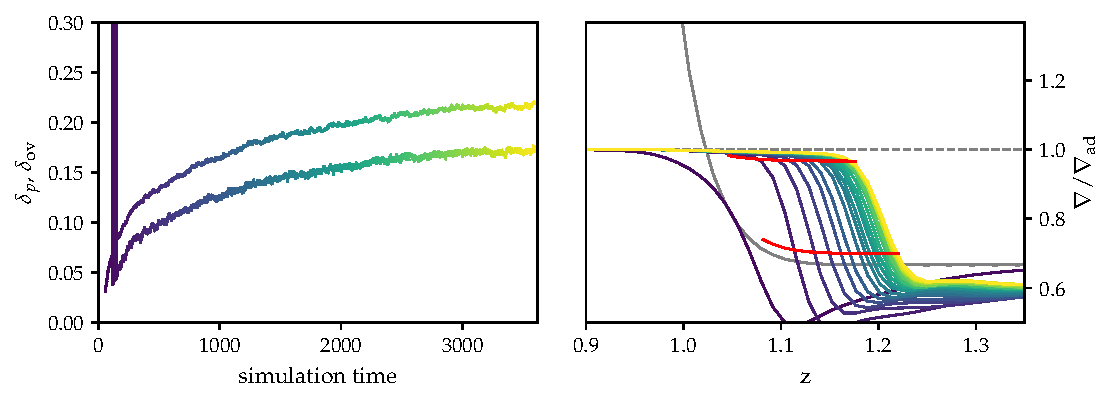
\includegraphics[width=\textwidth]{time_evolution.pdf}
\caption{
(left top panel) Shown is a trace of the PZ depth $\delta_{0.5}$ vs.~time, with convective freefall time units on the bottom x-axis and thermal diffusion time units (defined using the background $k$ in the radiative zone) on the upper x-axis.
We also show the time evolution of $f$ (left middle panel, defined in Eqn.~\ref{eqn:f_defn}) and $\xi$ (left bottom panel, defined in Eqn.~\ref{eqn:xi_defn}).
The vertical lines denote the times at which the traces first converge to within 1\% of their final values, which are denoted by solid horizontal lines.
(right panel) The vertical profile of $\justgrad/\gradad$ is plotted against height at regular time intervals.
The line color denotes the time, according to the time traces in the left panels.
The constant value of $\gradad$ is denoted by the horizontal dashed grey line, and the value of $\gradrad$ is denoted by the solid grey line.
The location of the Schwarzschild convective boundary is displayed as a vertical dashed black line and denotes the place where $\gradad = \gradrad$.
The top-of-PZ departure points (Eqn.~\ref{eqn:delta_p_measures}) are plotted over the profile evolution ($\delta_{0.1}$ and $\delta_{0.9}$ as red lines, $\delta_{0.5}$ as black lines).
\label{fig:time_evolution}
}
\end{figure*}



\subsection{Penetration depth measurements}
In our evolved simulations, we find that the penetrative region has a nearly adiabatic stratification $\justgrad \approx \gradad$.
In order to characterize the vertical extent of the penetrative region, we measure how drastically $\justgrad$ has departed from $\gradad$.
We define the difference between the adiabatic and radiative gradient,
\begin{equation}
\Delta\justgrad \equiv \gradad(z) - \gradrad(z).
\end{equation}
We measure penetration and overshoot depths in terms of ``departure points,'' or heights at which the realized temperature gradient $\justgrad$ has evolved away from the adiabatic $\gradad$ by some fraction $h < 1$.
Specifically,
\begin{equation}
L_s + \delta_{h} = \rm{max}(z) \,\,\mid\,\, \justgrad > (\gradad - h\,\Delta\justgrad).
\label{eqn:delta_p_measures}
\end{equation}
In this work, we measure the 10\% ($\delta_{0.1}$, $h=0.1$), 50\% ($\delta_{0.5}$, $h=0.5$), and 90\% ($\delta_{0.9}$, $h=0.9$) departure points.
Using \citet{zahn1991}'s terminology, $\delta_{0.5}$ is the mean value of the top of the PZ while $\delta_{0.9} - \delta_{0.1}$ roughly represents the width of the ``thermal adjustment layer.''
We will simply refer to these as three different measures of the top of the PZ.
We find that these measurements based on the (slowly-evolving) thermodynamic profile are more robust and straightforward than many previous dynamically-based prescriptions \citep[see e.g.,][for a nice discussion]{pratt_etal_2017}.

\begin{figure*}[t]
\centering
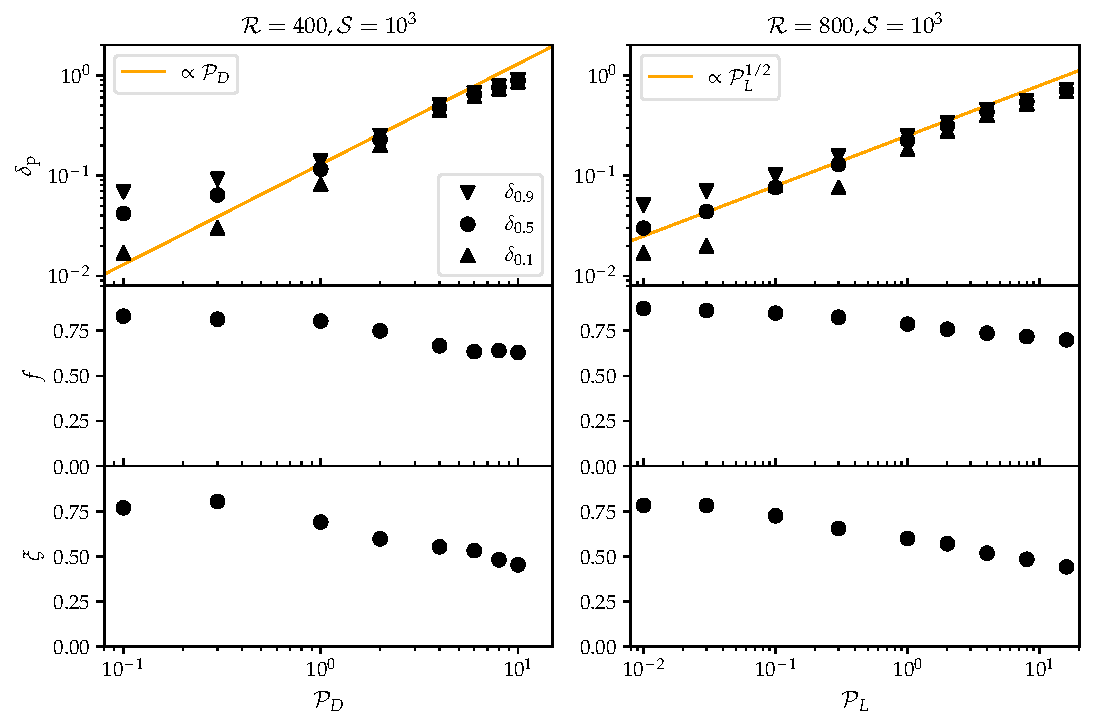
\includegraphics[width=\textwidth]{parameters_vs_p.pdf}
\caption{
Results from simulations with a Schwarzschild boundary characterized by a discontinuous conductivity (left, Case I, $k$ defined by Eqn.~\ref{eqn:sim_discontinuous_k}) and with a discontinuous conductivity gradient (right, Case II, $k$ defined by Eqn.~\ref{eqn:sim_linear_k}).
The top panels show the measured penetration depths according to Eqn.~\ref{eqn:delta_p_measures}.
The Case I penetration depths (upper left) vary roughly linearly with $\mP$, in line with the prediction of Eqn.~\ref{eqn:discontinuous_prediction}.
The Case II penetration depths (upper right) vary roughly like $\sqrt{\mP}$, in line with the prediction of Eqn.~\ref{eqn:linear_prediction}.
In the middle panels, we measure the evolved value of $f$ according to Eqn.~\ref{eqn:f_defn}.
We generally find values of $f \in [0.5, 0.9]$, and changes in $f$ are secondary to changes in $\mP$ for determining penetration depths.
In the bottom panels, we measure the evolved values of $\xi$ according to Eqn.~\ref{eqn:xi_defn}.
We find characteristic values of $\xi \in [0.5, 0.75]$, suggesting that the falloff of the $\bar{\Phi}$ in the PZ is well described by a linear function (at high $\mP$ when $\xi = 1/2$), or by a cubic function (at low $\mP$ when $\xi \approx 3/4$).
\label{fig:parameters_vs_p}
}
\end{figure*}





\section{Results}
\label{sec:results}

\subsection{Qualitative description of simulation evolution}

%\begin{figure*}[t]
%\centering
%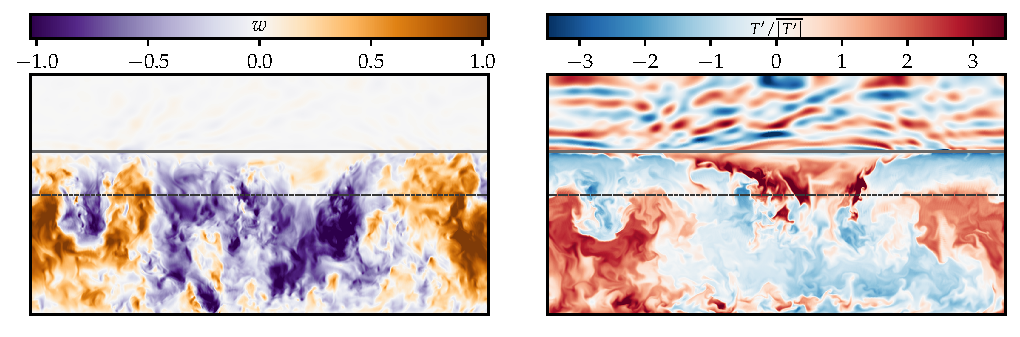
\includegraphics[width=\textwidth]{vertical_dynamics_panels.pdf}
%\caption{
%Displayed is an instantaneous snapshot of dynamics in a vertical slice through the simulation with $\mR = 6.4 \times 10^3$, $\mP_D = 4$ and $\mS = 10^3$.
%In both panels, the nominal Schwarzschild boundary of the convection zone where $\gradad = \gradrad$ is displayed as a dashed horizontal line, and the top of the penetrative zone ($\delta_{0.1}$) is shown by a solid horizontal line.
%(Left) The vertical velocity is shown; orange convective upflows extend far past the Schwarzschild boundary of the convection zone but stop abruptly where $\justgrad$ departs from $\gradad$.
%(Right) Temperature fluctuations are shown, normalized by their average magnitude at each height in order to clearly display all dynamical features.
%Unlike the vertical velocity, $T'$ shows distinctly different behavior in the CZ and PZ, switching sign at the Schwarzschild boundary of the convection zone.
%\label{fig:vertical_dynamics_panels}
%}
%\end{figure*}


In Fig.~\ref{fig:time_evolution}, we show the time evolution of a Case I (discontinuous conductivity) simulation with $\mR = 400$, $\mS = 10^3$, and $\mP_D = 4$ whose initial conditions roughly set $\justgrad = \gradad$ in the convection zone ($z \lesssim 1$) and $\justgrad = \gradrad$ in the radiative zone ($z \gtrsim 1$).
In the top left panel, we display the measured extent of the penetrative region $\delta_{\rm{0.5}}$ vs.~time.
This region initially grows quickly over hundreds of freefall times, but this evolution slows down as the convective dynamics establish themselves and the final equilibration takes tens of thousands of convective overturn (freefall) times.
The evolution of the other parameters in our theory ($f$, $\xi$) are shown in the middle and bottom left panels of Fig.~\ref{fig:time_evolution}.
We plot their rolling mean, averaged over 200 freefall time units. 
We see that the values of $f$ and $\xi$ reach their final values ($f \approx 0.67$, $\xi \approx 0.58$) faster than the penetration zone evolves to its full depth.
We quantify this fast evolution by plotting a vertical line in each of the left three panels corresponding to the first time at which the rolling average converges to within 1\% of its final value (averaged over the final 1000 freefall times of the simulation and plotted as a grey horizontal line).
The evolved value of $f$ indicates that roughly 2/3 of the buoyancy work is dissipated in the bulk CZ, so that 1/3 is available for PZ dissipation and negative buoyancy work.
The evolved value of $\xi$ indicates that the shape of dissipation in the PZ is slightly steeper than linear.

In the right panel of Fig.~\ref{fig:time_evolution}, we display the realized profile of $\justgrad/\gradad$ in our simulations at regular time intervals, where the color of the profiles corresponds to time, as in the left panels.
$\gradad$ is plotted as a dashed horizontal line while $\gradrad$ is plotted as a grey solid line which decreases with height around $z \approx 1$ and satures to a constant above $z \gtrsim 1.1$.
The location of the Schwarzschild boundary, $L_s$, is overplotted as a black vertical dashed line and does not evolve over the course of the simulation.
We note that the Schwarzschild boundary does not move over the course of our simulation, so the extention of the convection zone past this point is true penetration and not the result of entrainment-induced changes in the Schwarzschild (or Ledoux) convective boundaries.
The traces of $\delta_{0.1}$ and $\delta_{0.9}$ are plotted as red lines while that of $\delta_{0.5}$ is plotted as a black line.
We see that the fast initial evolution establishes a sizeable PZ (denoted by purple $\justgrad$ profiles), but its final equilibration slows down (indicated by the separation between the purple, green, and yellow profiles decreasing over time).
%This occurs in part because the flattening of $\justgrad < \gradrad$ above the penetrative zone increases the effective value of $N^2$ and thus the stiffness at the PZ-RZ boundary; however, this long evolution occurs on timescales similar to the thermal diffusion time in the RZ.

We note that this long evolution is extremely computationally costly; for this modest simulation (256x64$^2$ coefficients), this evolution represents roughly 20 days of evolution on 1024 cores for a total of $\sim$500,000 cpu-hours.
It is not feasible to perform simulations of this length for a full parameter space study, and so we accelerate the evolution of the bulk of the simulations in this work.
To do so, we take advantage of the nearly monotonic nature of the evolution of $\delp$ vs.~time displayed in Fig.~\ref{fig:time_evolution}.
We measure the instantaneous values of $(\delta_{0.1}, \delta_{0.5}, \delta_{0.9})$, as well as their instantaneous time derivatives.
Using these values, we take a large ``time step'' forward, advancing the values of $\delp$ according to their current trend.
While doing so, we preserve the width of the transition from the PZ to the RZ, and we also adjust the solution so that $\justgrad = \gradrad$ in the RZ, effectively equilibrating the RZ instantaneously.
For details on precisely how this procedure is carried out, see Appendix \ref{app:accelerated_evolution}.



%In Fig.~\ref{fig:vertical_dynamics_panels}, we display instantaneous vertical slices through a turbulent simulation with $\mR = 6.4 \times 10^3$, $\mP_D = 4$ and $\mS = 10^3$ with a coefficient resolution of 384$^3$ in an equilibrated state (this is the same $\mP_D$ and $\mS$ as in Fig.~\ref{fig:time_evolution}, but higher $\mR$).
%We see that strong convective dynamics (viewed in the left vertical velocity panel) extend beyond the Schwarzschild boundary of the convection zone (horizontal dashed grey line) into a penetration zone.
%Above the PZ, there is a dynamically distinct stable radiative zone with negligible vertical velocity (above the solid horizontal line).
%On the right, we see that hot upwellings in the convection zone are turned into cold upwellings in the PZ as a result of effective cooling from the sharp change in $k$ around the Schwarzschild boundary of the convection zone.
%These upwellings impinge upon the stable radiative zone and excite gravity waves, but our focus in this work is on the nature of the PZ where convective velocities and temperature anomalies are generally oppositely signed.

\begin{figure*}[t]
\centering
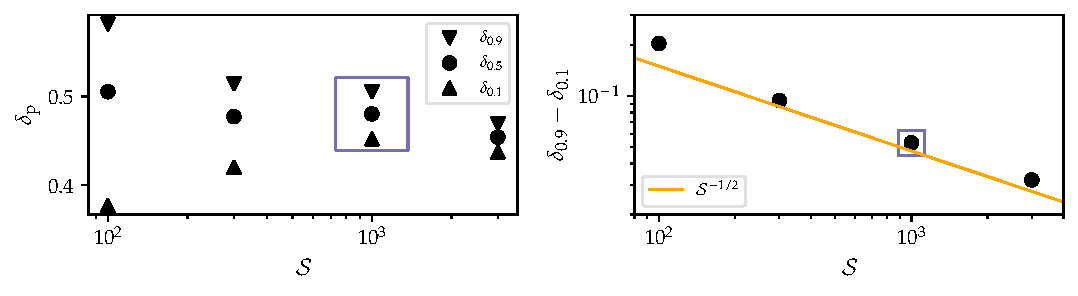
\includegraphics{parameters_vs_s.pdf}
\caption{
(Left panel) Penetration depths are shown as a function of stiffness for simulations with a discontinuous conductivity.
While the width of the transition layer from the adiabatic PZ to the stable RZ shrinks as a function of $\mS$, the mean penetration depth ($\delta_{0.5}$) is roughly constant.
(Right panel) The width of the thermal transition layer ($\delta_{0.9} - \delta_{0.1}$) is shown as a function of stiffness.
We roughly observe a $\mS^{-1/2}$ scaling, similar to that expected by e.g., \citet{korre_etal_2019}.
\label{fig:parameters_vs_s}
}
\end{figure*}




\subsection{Dependence on $\mP$}
We find that the depth of the penetration zone is strongly dependent on $\mP$.
In the upper two panels of Fig.~\ref{fig:parameters_vs_p}, we plot measured values of the penetration depth ($\delta_{0.1}$, $\delta_{0.5}$, $\delta_{0.9}$ from Eq.~\ref{eqn:delta_p_measures}) from Case I simulations (discontinuous $k$, upper left) and Case II simulations (discontinuous $\partial_z k$, upper right).
The fixed values of $\mR$ and $\mS$ are shown above these panels.
We find that the leading-order $\mP$ scaling predictions of Eqns.~\ref{eqn:discontinuous_prediction} \& \ref{eqn:linear_prediction} describe the data extremely well (orange lines).
At small values of $\mP$ we see somewhat weaker scalings than these predictions; this is caused by the fact that the profiles of $k$ and $\partial_z k$ are not truly discontinuous but jump from one value in the CZ to another in the RZ over a finite width (see e.g., the $\gradrad$ profile in Fig.~\ref{fig:time_evolution} \& Sec.~\ref{sct:numerics}).
At large values of $\mP$, penetration depths begin to fall off of these predicted scaling laws, which makes sense: in this regime, dissipation dominates over buoyancy in the PZ and PZ depths saturate.

The middle and bottom panels of Fig.~\ref{fig:parameters_vs_p} demonstrate that it is reasonable but imprecise to assume that $f$ and $\xi$ are constant as a function of $\mP$.
We find that $f$ has slightly smaller values in the Case I simulations (left) than in the Case II simulations (right).
We measure characteristic values of $f \in [0.6, 0.9]$, signifying that 60-90\% of the buoyant work is balanced by dissipation in the convection zone, depending on the simulation.
We note a weak trend where $f$ decreases as $\mP$ increases.
Most of this trend can be explained by slight decreases in the CZ velocities and corresponding decreases in the dissipation.
We speculate that when $\mP$ is small, the PZ-RZ boundary (which acts like a wall, left panel of Fig.~\ref{fig:vertical_dynamics_panels}) efficiently deflects convective velocities sideways resulting in increased bulk-CZ velocities.
As $\mP$ grows, the velocities have access to an extended PZ in which to buoyantly break before deflection, resulting in slightly lower bulk velocities.
A similar trend of $\xi$ decreasing as $\mP$ increases can be seen.
This makes sense: $\xi$ is a measure of how different dissipative dynamics are in the CZ compared to the PZ.
As the size of the PZ grows, dynamics have the space to change appreciably from their bulk-CZ properties, and so $\xi$ shrinks.

\subsection{Dependence on $\mS$}

We find that the depth of the penetration zone is weakly dependent on $\mS$.
In the left panel of Fig.~\ref{fig:parameters_vs_s}, we plot the penetration depth of a few discontinuous-$k$ simulations with $\mP_D = 4$ and $\mR = 400$ but with different values of $\mS$.
We find that the mean penetration depth $\delta_{0.5}$ varies only weakly with changing $\mS$, but that the values of $\delta_{0.1}$ and $\delta_{0.9}$ vary somewhat strongly.
In other words, the smooth transition region in which $\justgrad$ varies from $\gradad$ in the PZ to $\gradrad$ in the RZ becomes narrower as $\mS$ increases.
To quantify this effect, we plot $\delta_{0.9} - \delta_{0.1}$ in the righthand panel of Fig.~\ref{fig:parameters_vs_s}.
We find that the width of this region roughly varies according to a $\mS^{-1/2}$ scaling law, which is reminiscent of the pure-overshoot laws described by \citet{korre_etal_2019}.
%This suggests that the evolved profile of a convecting region can be described by a penetration zone (described by e.g., $\mP$, $f$, and $\xi$) with a thin overshooting region (described by $\mS$) within the transition between the PZ and RZ.

We note briefly that if the enstrophy, $\omega^2$ in the convection zone exceeded the value of the square buoyancy frequency $N^2$ in the radiative zone, the gravity waves in the RZ became nonlinear.
As a result, we have restricted the simulations in this study to relatively large (yet modest compared to astrophysical values) of $10^{2} \leq \mS < 10^4$ in order to ensure $N^2 > \omega^2$ even in our turbulent cases.

\begin{figure*}[t]
\centering
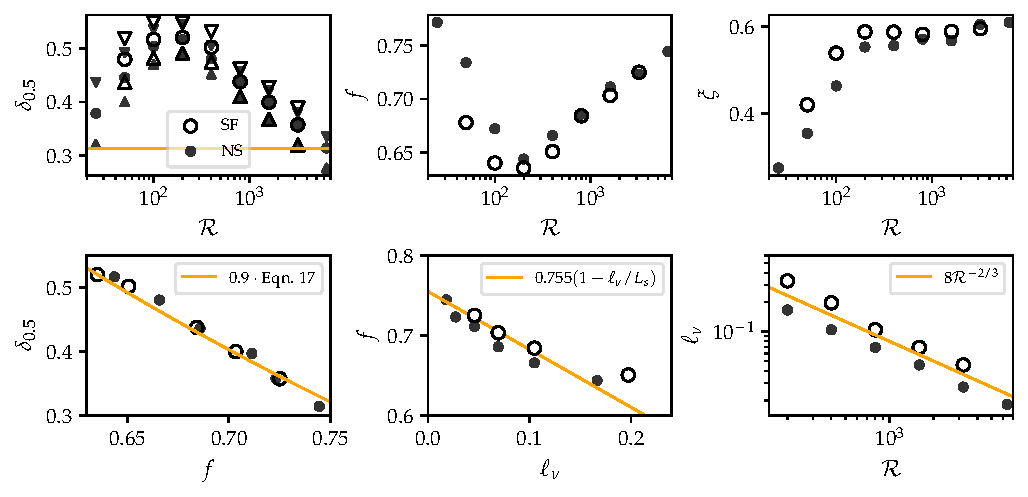
\includegraphics[width=\textwidth]{parameters_vs_re.pdf}
\caption{
(Upper left panel) Penetration depths are shown as a function of increasing Reynolds number ($\mR$) for simulations with a discontinuous conductivity.
We plot results both for cases with stress-free boundary conditions (SF) and no-slip boundary conditions (NS).
In both cases, we see a roughly logarithmic decrease of $\delp$ with $\mR$.
(Upper middle panel) We similarly see increases in the value of $f$ with $\mR$, although perhaps this measurement is leveling off at high values of $\mR$.
(Upper right panel) We do not see large changes in the value of $\xi$ as $\mR$ increases, suggesting that the nature of dissipation in the PZ is not appreciably changing.
(Lower left panel) In summary, we see a strong correlation between $\delta_{0.5}$ and $f$.
(Lower middle panel) Changes in $f$ are roughly linearly proportional to the depth of the viscous boundary layer, $\ell_\nu$, at the bottom of the domain, at least for the open-circle SF cases.
This makes sense, as more of the convective domain is available for the convective flows to dissipate energy.
(Lower right panel) The viscous boundary layer follows a classical scaling laws seen in Rayleigh-B\'{e}nard convection, and so we anticipate that the trend in $\delta_{0.5}$ vs $\mR$ should saturate as $\delta_{\nu} \rightarrow 0$ and $f$ saturates.
\label{fig:parameters_vs_re}
}
\end{figure*}





\subsection{Dependence on $\mR$}

We find that the depth of the penetration zone is weakly dependent on $\mR$.
In the upper left panel of Fig.~\ref{fig:parameters_vs_re}, we find a logarithmic decrease in the penetration depth with the Reynolds number.
In order to understand how this could happen at fixed $\mP$, we plot the output values of our parameterized values $f$ (upper middle) and $\xi$ (upper right).
We find that $f$ increases with increasing $\mR$, but is perhaps leveling off as $\mR$ becomes large.
We find that $\xi$ does not increase strongly with $\mR$ except for in the case of laminar simulations with $\mR < 200$.
Indeed, the variation of $\delp$ with $\mR$ can be seen as a variation of $\delp$ with $f$ in the bottom left panel.
We find that this is true both for simulations with stress-free dynamical boundary conditions (open symbols, SF) and for no-slip conditions (closed symbols, NS).

In order to understand this better, we note that the dissipation profile can reasonably be approximated as a constant value in the CZ and zero in the bottom viscous boundary layer.
We have visualized a NS dissipation profile in the bottom panel of Fig.~\ref{fig:theory_profiles}; SF simulations look similar in the bulk, but drop towards zero at the bottom boundary rather than reaching a maximum.
We can model the dissipation in the $f$ definition (Eqn.~\ref{eqn:f_defn}) as a constant in the bulk and zero in the boundary layer,
\begin{equation}
\int_{\rm{CZ}} \bar{\Phi}\,dz \approx C \left( 1 - \frac{\ell_\nu}{L_s}\right)
\,\,\Rightarrow\,\,
f \propto \left(1 - \frac{\ell_\nu}{L_s}\right),
\end{equation}
where $C$ is a constant and $\ell_\nu$ is the boundary layer depth.
In this model, we expect the dissipation and therefore $f$ to vary linearly with the viscous boundary layer depth.
We take the value of $\ell_\nu$ to be the height of the extremum of the viscous portion of the kinetic energy flux $\bar{\mathcal{F}}$ near the boundary.
In the bottom middle panel of Fig.~\ref{fig:parameters_vs_re}, we find that $f \approx 0.755(1 - 2\ell_\nu/L_s)$ is a decent description of the high-$\mR$ behavior of these simulations.
The additional factor of 2 arises because of how we find the boundary layer depth (the extremum of the viscous flux likely occurs halfway through the boundary layer spatially).
We find that this is a slightly better description for the SF simulations than the NS simulations; NS simulations have maximized dissipation in the bounary layer, and therefore this model poorly describes them from a phenomenological perspective.
In the bottom right panel of Fig.~\ref{fig:parameters_vs_re}, we demonstrate that the depth of the viscous boundary layer follows classical scaling laws from Rayleigh-B\'{e}nard convection\footnote{
If you assume the Nusselt Number dependence on the Rayleigh number is throttled by the boundaries, Nu $\propto$ Ra$^{1/3}$ (as is frequently measured), and the Reynolds number is Re $\propto$ Ra$^{1/2}$, you retrieve Nu $\propto$ Re$^{2/3}$. 
The Nusselt number generally varies like the inverse of the boundary layer depth, Nu $\propto$ $\delta^{-1}$, and so we expect $\delta_{\nu} \propto \mR^{-2/3}$.
} \citep{ahlers_etal_2009, goluskin2016}.
Combining these trends, we expect $f \propto \mR^{-2/3}$, and so expect the changes in $f$ and $\delp$ to level off as $\mR$ increases to high values in the astrophysical regime.

Indeed, we use the fitted function of $f$ from the bottom middle panel, along with Eqn.~\ref{eqn:discontinuous_prediction}, to estimate $\delta_{0.5}$ in the bottom left panel, and we overplot that as a line.
We need to multiply this equation by a factor of 0.9, which accounts for some differences between the simulations and the idealized ``discontinuous flux'' theoretical model.
First, due to internal heating and the finite width of the conductivity transition around the Schwarzschild boundary, the convective flux is not truly constant through the full depth of the CZ.
Thus, we expect $L_{\rm{CZ}}$  in Eqn.~\ref{eqn:discontinuous_prediction} to be smaller than 1.
Furthermore, the theory is derived in the limit of an instantaneous tarnsition from $\gradad$ to $\gradrad$ where $\delta_{0.1} = \delta_{0.5} = \delta_{0.9}$; our simulations have a finite transition width.
Despite these subtle differences, we find good agreement.

Using the value of $f = 0.755$ expected at $\ell_\nu = 0$, we calculate that we expect $\delta_{0.5} \approx 0.31$ for $\mR \rightarrow \infty$ and overplot this as a horizontal orange line on the upper left panel of Fig.~\ref{fig:parameters_vs_re}.
This value is coincidentally very near the value of $\delta_{0.5}$ achieved in our highest-$\mR$ simulations.
Unfortunately, we cannot probe more turbulent simulations than these.
We can only run the $\mR = 6.4 \times 10^{3}$ simulations for a few hundred freefall times.
Our accuracy in measuring results from these simulations is limited by the long evolutionary timescales of these simulations (see Fig.~\ref{fig:time_evolution}).
Even accounting for our accelerated evolutionary procedure, we can only be confident that the PZ depths of these simulations are converged to within a few percent.
Future work should aim to better understand the trend of PZ depth with turbulence.
However, the displayed relationships between $\delp$ and $f$, $f$ and $\ell_\nu$, and $\ell_\nu$ and $\mR$ --- all of which are effects we largely understand --- suggest that PZ depths should saturate at high $\mR$.




\section{A modified solar model}
\label{sec:solar_model}
Our simulation results present a strong case for the validity of a flux- and dissipation-based model of convective penetration, similar to those considered by \citet{zahn1991} and \citet{roxburgh1989}.
In general, out of the simulations presented in this work, we expect the simulation with $\mP_L = 1$ (a linear radiative conductivity profile) to be the most representative of conditions near a stellar convective boundary.
In this simulation, we found $f \approx 0.8$ and $\xi \approx 0.6$.
We note that Fig.~\ref{fig:parameters_vs_re} suggests that $f$ could increase by $\sim 0.1$ as $\mR$ increases into the stellar regime but $\xi$ probably doesn't change much.
As such, we take $f = 0.9$ and $\xi = 0.6$ as first-guess values for our theory of convective penetration in stellar regimes.
These values should of course be confirmed and tuned in more realistic stellar settings which include spherical geometry and realistic density stratifications.

In spherical geometry, if the horizontal averages of Eqn.~\ref{eqn:integral_constraint} are replaced with integrals over latitude and longitude, the relevant integral constraint for convective penetration can be described in terms of the convective luminosity,
\begin{equation}
\int |\alpha| g L_{\rm{conv}}\,dr =   \int_V \rho_0 \Phi\,dV,
\end{equation}
where $L_{\rm{conv}} = 4\pi\rho_0 r^2 \bar{F_{\rm{conv}}}$, $r$ is the radial coordinate, and we write the RHS as a volume integral.
We next define $f$ in the same way as in Eqn.~\ref{eqn:f_defn} and define $\xi$ similarly to Eqn.~\ref{eqn:xi_defn},
\begin{equation}
\int_{\rm{PZ}} \rho_0 \Phi \,dV = \xi \frac{V_{\rm{PZ}}}{V_{\rm{CZ}}}\int_{\rm{CZ}}\rho_0 \Phi \, dV,
\end{equation}
where $V_{\rm{PZ}}$ and $V_{\rm{CZ}}$ are the volumes of the CZ and PZ respectively.
This is the generalized version of Eqn.~\ref{eqn:xi_defn} outside of the assumption of a plane-parallel atmosphere.
A first-guess at the equivalent of Eqn.~\ref{eqn:theory_fraction} in stellar contexts is
\begin{equation}
-\frac{\int_{\rm{PZ}} L_{\rm{conv}}\,dr}{\int_{\rm{CZ}} L_{\rm{conv}}\,dr} + f \xi \frac{V_{\rm{PZ}}}{V_{\rm{CZ}}} = (1 - f),
\label{eqn:mesa_eqn}
\end{equation}

We implemented Eqn.~\ref{eqn:mesa_eqn} in MESA (see Appendix \ref{app:mesa} for details) and computed a standard solar model with $f = 0.9$ and $\xi = 0.6$ to determine an extremely rough first-estimate of how the dissipative treatment presented in this work might adjust a familiar stellar model.
We chose a value of $\xi = 1$ as it is the most conservative choice and should generally result in smaller penetration zones, and because it is unclear how our plane-parallel intuition for $\xi$ in this study maps into spherical geometry.
We of course note that the work that we presented here is done under the incompressible approximation and does not include the many complications of stellar convection like density stratification, sphericity, rotation, magnetism, etc.
We present this model as a proof of concept and to inspire further work.

In Fig.~\ref{fig:mesa} we display the profile of X quantity at the base of a solar model using a penetrative zone (as described above) and using X classical prescription.
Note the differences in this thing and that thing.

TODO: Implement this in MESA, and make a simple figure comparing some solar profiles near the base of the CZ!

We find a convection zone which extends an additional $X H_p$ beneath the nominal Schwarzschild base of the convection zone.
Early studies suggest that the maximum depth of a PZ should be 0.1 $H_p$ \citep{basu_etal_1994}.
More recent work puts tighter helioseismic constraints on observations of $0.05 H_p$, which compares to our model in X way \citep[see e.g., section 7.2.1 of][]{basu2016}.
However, the recent simulations of \citet{kapyla2019} suggest an overshooting depth of $0.2 H_p$ at the base of the solar convection zone.
We hope to improve this model and stuff in future work, please hang out with us and make it better.


\section{Discussion}
\label{sec:discussion}
In this work, we presented dynamical simulations of convective penetration, in which convection flattens $\justgrad \rightarrow \gradad$ beyond the Schwarzschild convective boundary.
To understand these simulations, we used an integral constraint \citep[reminiscent of][]{roxburgh1989} and flux-based arguments \citep[similar to][]{zahn1991} to derive a parameterization of convective penetration according to the convective flux and viscous dissipation.
In doing so, we have laid down the first steps (Eqns.~\ref{eqn:theory_fraction} \& \ref{eqn:mesa_eqn}) towards incorporating convective penetration into stellar structure codes.
We parameterized the viscous dissipation into a bulk-CZ portion ($f$) and a portion in the extended penetrative region ($\xi$), and derived predictions for how the depth of a penetrative region, $\delp$, should scale with these measurable parameters and a new flux-based ``penetration parameter'' $\mP$.
We designed and analyzed two sets of simulations which showed good agreement with these theoretical predictions.
We furthermore examined briefly what the impliciations of this theory could be for a simple solar model.

Our simulation results suggest that stellar convection zones should be bounded by appreciably large penetration zones.
In extreme cases, we observe penetration zones which are as large as the convection zones they accompany; however, for realistic stellar values ($\mP \approx 1$), we find that they may be as large as 20-30\% of the convective zone length scale ($\sim$the mixing length).

The simulations we presented in this work were the simplest possible simulations to try to test the basic tenets of our theory.
In particular, they demonstrate that the shape of the flux near the convective boundary and the viscous dissipation together fully determine the depth of the penetration zone.
The precise values of the parameters $f$ and $\xi$ achieved in natural, turbulent, fully compressible, spherical stellar convection may be different from those presented in e.g., Fig.~\ref{fig:parameters_vs_p} here.
Future work should aim to understand how these parameters and the theory presented in e.g., Eqn.~\ref{eqn:mesa_eqn} change when these realistic effects are taken into account.

Furthermore, it is important to note that stellar opacities, and thus stellar conductivities, are functions of thermodynamic variables rather than radial location.
As a result, the formation of a penetration zone will in turn affect the conductivity profile and $\gradrad$, which will in turn affect the location of the Schwarzschild boundary and the estimate of how deep the penetration zone should be.
Future studies should follow e.g., \citet{kapyla_etal_2017} and implement realistic opacity profiles which evolve self-consistently with the thermodynamic state in order to understand how these effects feedback into one another.

An additional complication is that stellar fluid dynamics exist in the regime of Pr$\,\ll1$ \citep{garaud2021}.
Dynamics in this regime may be different from those in the regime of Pr $\lesssim 1$ that we studied here, which in theory could affect $f$ and $\xi$.
Recently, \citet{kapyla2021} found that convective flows exhibited more penetration at low Pr than high Pr.
Future work should aim to understand whether $f$ and $\xi$ depend strongly on $\Pran$ in the turbulent regime.

Two other interesting complications in stellar contexts are rotation and magnetism.
In the rapidly rotating limit, rotation creates quasi-two-dimensional flows, which could affect the length scales on which dissipation acts and thus modify $f$.
Furthermore, magnetism adds an additional ohmic dissipation term, which could in theory drastically change our hydrodynamical measurement of $f$.

Finally, we note that our work here assumes a uniform composition through the convective and radiative region.
Frequently within stars, convective boundaries coincide with discontinuities in composition profiles \citep{salaris_cassisi_2017}.
Future work should also aim to determine if stabilizing composition gradients can prevent the formation of penetration zones seen here (as in Fig.~\ref{fig:time_evolution}).

In summary, we have unified \citet{roxburgh1989}'s integral constraint with \citet{zahn1991}'s theory of flux-dependent penetration into a parameterized theory of convective penetration.
We tested this theory with simulations and found good agreement between the theory and our simulations.
In future work, we will aim to more robustly implement this theory into MESA and use simulations to test some of the complicating factors we discussed here.





\begin{acknowledgments}
We'd like to thank Keaton Burns, Matt Browning, Matteo Cantiello and Kyle Augustson for useful discussions and questions which improved the content of this manuscript.
EHA is funded as a CIERA Postdoctoral fellow and would like to thank CIERA and Northwestern University. 
We acknowledge the hospitality of Nordita during the program ``The Shifting Paradigm of Stellar Convection: From Mixing Length Concepts to Realistic Turbulence Modelling," where the groundwork for this paper was set.
Computations were conducted with support from the NASA High End Computing (HEC) Program through the NASA Advanced Supercomputing (NAS) Division at Ames Research Center on Pleiades with allocation GID s2276.
\end{acknowledgments}


\appendix

\section{Accelerated Evolution}
\label{app:accelerated_evolution}
As demonstrated in Fig.~\ref{fig:time_evolution}, the time evolution of simulations which start from a state based on the Schwarzschild criterion can be prohibitively long.
In \citet{anders_etal_2018}, we explored the long time evolution of simple convective simulations and found that fast-forwarding the evolution of a convective simulation's internal energy and thermal structure can be done accurately.
This can be done because the convective dynamics converge rapidly even if the thermal profile converges slowly.
This same separation of scales is observed in the left panels of Fig.~\ref{fig:time_evolution} in this work, and so similar techniques should be applicable.

In this work, we accelerate the evolution of of our simulations in order to more quickly determine the final size of the evolved penetration zones according to the following algorithm.
\begin{enumerate}
\item Once a simulation has a volume-averaged Reynolds number greater than 1, we wait 10 freefall times to allow dynamical transients to pass.
\item We measure the departure points ($\delta_{0.1}$, $\delta_{0.5}$, $\delta_{0.9}$) every freefall time, and store this information for 30 freefall times.
\item We linearly fit each of the departure points' evolution against time using NumPy's \texttt{polyfit} function.
We assume that convective motions influence $\delta_{0.1}$ and $\delta_{0.5}$ more strongly than $\delta_{0.9}$.
We measure the time-evolution of the convective front $\frac{d \delp}{dt}$ by averaging the slope of the linear fits for $\delta_{0.1}$ and $\delta_{0.5}$.
\item We take a large ``time step'' of size $\tau_{\rm{AE}}$ forward.
We calculate $\Delta \delta_p = \tau_{\rm{AE}} \frac{d \delp}{dt}$.
\begin{itemize}
\item If $\Delta \delta_p < 0.005$, we erase the first 15 time units worth of departure point measures and return to step 2 for 15 time units.
\item  If $\Delta \delta_p$ is large, we adjust the top of the PZ by setting $\delta_{0.5,\rm{new}} = \angles{\delta_{0.5}}_t + \Delta \delta_p$ (angles represent a time average).
If $|\Delta \delta_p| > 0.05$, we limit its value to 0.05.
We calculate the width of the thermal adjustment layer $d_w$ as the minimum of $\angles{\delta_{0.9} - \delta_{0.5}}_t$ and $\angles{\delta_{0.5} - \delta_{0.1}}_t$.
We adjust the mean temperature gradient to
\begin{equation}
\partial_z \overline{T} = -\gradad - H(z; \delta_{\rm{0.5,\rm{new}}}, d_w) \Delta\justgrad,
\label{eqn:initial_grad}
\end{equation}
where $H$ is defined in Eqn.~\ref{eqn:heaviside} and $\Delta\justgrad = \gradrad - \gradad$.
We also multiply the temperature perturbations and full convective velocity field by $(1 - H(z; 1, 0.05))$.
This sets all fluctuations above the nominal Schwarzschild convection zone to zero, thereby avoiding any strange dynamical transients caused by the old dynamics at the radiative-convective boundary (which has moved as a result of this process).
\end{itemize}
\item We restart from step 1.
\end{enumerate}
In general, the initial profile of $\bar{T}$ that we use when we start our simulations is given by Eqn.~\ref{eqn:initial_grad} with a value $\delta_{0.5,\rm{new}} \geq 0$.
We then evolve $\bar{T}$ towards a statistically stationary state using the above algorithm and standard timestepping.
If a simulation returns to step 2 from step 4 ten times over the course of its evolution, we assume that it has converged near its answer, stop this iterative loop, and allow the simulation to timestep normally.
Additionally, in some simulations, we ensure that this process occurs no more than 25 times.
This process effectively removes the long diffusive thermal evolution on display in the upper left panel of Fig.~\ref{fig:time_evolution} by immediately setting the mean temperature profile to the radiative profile above the PZ.

In Fig.~\ref{fig:AE_time_figure}, we display the time evolution of $\delp$ and $f$ in Case I simulations with $\mS = 10^3$, $\mR = 400$, and $\mP_D = [1,2,4]$ simulations using black lines.
We overplot the evolution of simulations which use this accelerated evolution (AE) procedure using orange and green lines.
Time units on the x-axis are normalized in terms of the total simulation run time in order to more thoroughly demonstrate the evolutionary differences between standard timestepping and AE.
However, the AE simulations are much shorter: the vertical green-and-yellow lines demonstrate how long the AE simulation ran compared to the standard timestepping simulation (so for $\mP_D = 1$, the AE simulations only took $\sim 1/4$ as long; for $\mP_D = 2$, they took $\sim 1/8$ as long; for $\mP_D = 4$, they took $\sim 1/20$ as long).
AE simulations with orange lines start with PZ depths which are much larger than the final depth, while green line solution start with initial PZ depths which are smaller than the expected depth.
Regardless of our choice of initial condition, we find that this AE procedure quickly evolves our simulations to within a few percent of the final value.
After converging to within a few percent of the proper penetration zone depth, this AE procedure continues to iteratively ``jitter'' around the right answer until the convergence criterion we described above are met.
These jitters can be seen in the top panels of Fig.~\ref{fig:AE_time_figure}, where the solution jumps away from the proper answer in one AE iteration before jumping back towards it in the next iteration.
If the PZ depth continues to noticeably vary on timescales of a few hundred freefall times, we continue to timestep the simulations until the evolution of $\delp$ vs.~time has flattened.

\begin{figure*}[t]
\centering
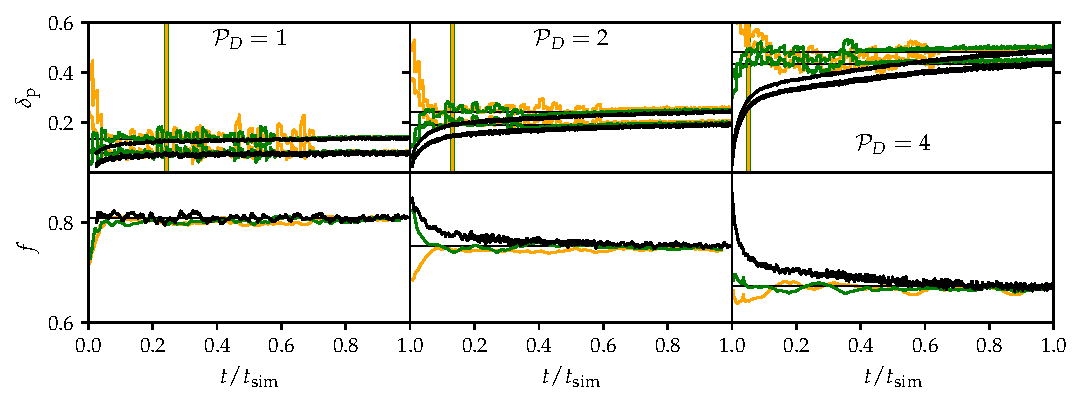
\includegraphics[width=\textwidth]{AE_time_figure.pdf}
\caption{
\label{fig:AE_time_figure}
(top row) Time traces of $\delta_{0.1}$ and $\delta_{0.9}$ for simulations which are computed using (black lines) standard timestepping, (orange lines) accelerated evolution with large initial values of $\delp$, and (green lines) accelerated evolution with small initial values of $\delp$.
The thin horizontal lines represent the final converged values from the standard timestepping simulations.
Accelerated evolution timesteps can be seen as discontinuities in the $\delp$ trace.
Once the procedure gets to within a few percent of the appropriate value, any large steps away from the ``correct'' solution are quickly reversed.
Time units are normalized by the total run time of the simulation.
All accelerated evolution simulations were run for $t_{\rm{sim}} = 3000$ freefall times.
The standard timestepping (black line) simulations were run for $t_{\rm{sim}} = 1.2 \times 10^4$ ($\mP_D = 1$), $t_{\rm{sim}} = 2.2 \times 10^4$ ($\mP_D = 2$), or $t_{\rm{sim}} = 5.7 \times 10^4$ ($\mP_D = 4$) freefall times.
The vertical green-and-yellow bars show the total length of the accelerated simulation in terms of the classic simulation; so the vertical lines in the upper right panel show that the accelerated simulation was converged after $\sim$ 5\% of the classic simulation.
(Bottom row) Same as top row, but where a rolling average of $f$ over 200 freefall times is shown.
}
\end{figure*}





\section{MESA implementation}
\label{app:mesa}
Here we describe a first implementation of Eqn.~\ref{eqn:mesa_eqn} in MESA \citep{paxton_etal_2011, paxton_etal_2013, paxton_etal_2015, paxton_etal_2018, paxton_etal_2019}.
We note that this impelementation is likely not universal or robust enough to be used in any stellar model, but it is robust enough to timestep stably and produce the results displayed in Sct.~\ref{sec:solar_model}.
Future work should improve upon this model.

To find the extent of the penetrative region, we override MESA's TODO routine for writing $\justgrad$ and instead have the solver follow these steps:
\begin{enumerate}
\item At each timestep, we find the location of the Schwarzschild convective boundary, $r_s$.
We measure the value of the mixing length $\lambda$ there, and choose a convection zone length scale $\ell_{\rm{CZ}} = \text{min}(\lambda, L_{\rm{CZ}})$, where $L_{\rm{CZ}}$ is the full depth of the Schwarzschild-unstable convective region.
We take the ``CZ'' integrals in Eqn.~\ref{eqn:mesa_eqn} to span radially from the Schwarzschild boundary to a depth $\ell_{\rm{CZ}}$ within the convection zone.
\item We calculate the buoyancy integral $\int_{\rm{CZ}} L_{\rm{conv}} dr$ and the convection zone volume $V_{\rm{CZ}}$.
\item Starting at the Schwarzschild boundary, we iteratively expand the size of the PZ until Eqn.~\ref{eqn:mesa_eqn} is satisfied.
For each radial bin $i$ below the convection zone, we calculate $\int_{\rm{PZ},i}L_{\rm{conv}} dr$ and $V_{\rm{PZ},i}$.
We evaluate the LHS of Eqn.~\ref{eqn:mesa_eqn} using those values.
If LHS $\geq$ RHS, we assume that the radial coordinate of bin $i$ is the boundary of the penetrative region.
\item We enforce $\justgrad \approx \gradad$ in the PZ by doing TODO.
\item We ensure that the transition from the PZ to the RZ is smooth.
Outside of the PZ, we model $\justgrad$ as TODO.
\end{enumerate}

Using this procedure with $f = 0.8$ and $\xi = 1$, and timestepping a solar model to the age of the current Sun ($\sim$ 4.5 Gyr), we find the profile displayed in Sec.~\ref{sec:solar_model}.


\newpage
\section{Table of simulation parameters}
\label{app:simulation_table}

\begin{deluxetable*}{c c c c c c c c c c}
\tabletypesize{\footnotesize}
\caption{Table of simulation information
\label{table:simulation_info}
}
\tablehead{
\colhead{Type} 	& \colhead{$\mP$}	& \colhead{$\mS$}	& \colhead{$\mR$}	& \colhead{$nz \times (nx \times ny)$}	&	\colhead{$t_{\rm{sim}}$}	&	\colhead{$(\delta_{0.1}, \delta_{0.5}, \delta_{0.9})$}	& \colhead{$f$}	& \colhead{$\xi$}	& \colhead{$\angles{u}$}
}
\startdata
\multicolumn{3}{l}{\textbf{``Standard timestepping'' simulations}}\\
D	& 1	& $10^3$	& $4 \times 10^2$	& 256$\times$64$^2$	& 12347	& ($0.078, 0.112, 0.136$)	& 0.81	& 0.70	& 0.61 \\
D	& 2	& $10^3$	& $4 \times 10^2$	& 256$\times$64$^2$	& 22593	& ($0.191, 0.220, 0.242$)	& 0.75	& 0.62	& 0.62 \\
D	& 4	& $10^3$	& $4 \times 10^2$	& 256$\times$64$^2$	& 57170	& ($0.434, 0.461, 0.483$)	& 0.67	& 0.58	& 0.62 \\
\hline
\multicolumn{3}{l}{\textbf{``Accelerated Evolution'' simulations}}\\
D		& 0.1,  & $10^3$    & $4 \times 10^2$   & 256$\times$64$^2$	 	& 4561 	& ($0.017, 0.042, 0.069$)	&  0.83	&  0.77	& 0.59 \\
D		& 0.3,  & $10^3$    & $4 \times 10^2$   & 256$\times$64$^2$	 	& 4681 	& ($0.030, 0.064, 0.092$)	&  0.81	&  0.80	& 0.62 \\
D		& 1,    & $10^3$    & $4 \times 10^2$   & 256$\times$64$^2$	 	& 3000 	& ($0.082, 0.116, 0.140$)	&  0.80	&  0.69	& 0.62 \\
D		& 2,    & $10^3$    & $4 \times 10^2$   & 256$\times$64$^2$	 	& 5000 	& ($0.199, 0.228, 0.252$)	&  0.75	&  0.60	& 0.64 \\
D		& 4,    & $10^3$    & $4 \times 10^2$   & 256$\times$64$^2$	 	& 5000 	& ($0.452, 0.480, 0.505$)	&  0.67	&  0.55	& 0.62 \\
D		& 6,    & $10^3$    & $4 \times 10^2$   & 256$\times$64$^2$	 	& 6000 	& ($0.620, 0.647, 0.667$)	&  0.64	&  0.53	& 0.60 \\
D		& 8,    & $10^3$    & $4 \times 10^2$   & 512$\times$128$^2$	& 4357 	& ($0.731, 0.757, 0.778$)	&  0.64	&  0.48	& 0.59 \\
D		& 10,   & $10^3$    & $4 \times 10^2$   & 512$\times$128$^2$	& 4226 	& ($0.857, 0.884, 0.903$)	&  0.63	&  0.45	& 0.59 \\
D   	& 4		& $10^3$			& 25				& 256$\times$16$^2$ 	& 3000	& (0.321, 0.379, 0.437)	& 0.77	& 0.27	& 0.34 \\
D   	& 4		& $10^3$			& 50				& 256$\times$32$^2$ 	& 3000	& (0.398, 0.442, 0.487)	& 0.73	& 0.36	& 0.42 \\
D   	& 4		& $10^3$			& $1 \times 10^2$	& 256$\times$32$^2$ 	& 3000	& (0.469, 0.503, 0.534)	& 0.67	& 0.46	& 0.48 \\
D   	& 4		& $10^3$			& $2 \times 10^2$	& 256$\times$64$^2$ 	& 3000	& (0.485, 0.515, 0.542)	& 0.65	& 0.55	& 0.55 \\
D   	& 4		& $10^3$			& $8 \times 10^2$	& 256$\times$128$^2$	& 3000	& (0.407, 0.434, 0.455)	& 0.69	& 0.57	& 0.68 \\
D   	& 4		& $10^3$			& $1.6 \times 10^3$	& 256$\times$128$^2$	& 3000	& (0.366, 0.397, 0.419)	& 0.71	& 0.57	& 0.72 \\
D   	& 4		& $10^3$			& $3.2 \times 10^3$	& 256$^3$				& 2469	& (0.313, 0.350, 0.372)	& 0.73	& 0.60	& 0.75 \\
D   	& 4		& $10^3$			& $6.4 \times 10^3$	& 384$^3$				& 414 	& (0.277, 0.314, 0.335)	& 0.74	& 0.62	& 0.76 \\
D/SF	& 4		& $10^3$			& 50				& 256$\times$16$^2$ 	& 5000	& (0.435, 0.477, 0.516)	& 0.68	& 0.42	& 0.50 \\
D/SF	& 4		& $10^3$			& $1 \times 10^2$	& 256$\times$32$^2$ 	& 5000	& (0.482, 0.516, 0.547)	& 0.64	& 0.54	& 0.57 \\
D/SF	& 4		& $10^3$			& $2 \times 10^2$	& 256$\times$32$^2$ 	& 5000	& (0.490, 0.520, 0.547)	& 0.63	& 0.59	& 0.64 \\
D/SF	& 4		& $10^3$			& $4 \times 10^2$	& 256$\times$64$^2$ 	& 8000	& (0.474, 0.502, 0.531)	& 0.65	& 0.59	& 0.69 \\
D/SF	& 4		& $10^3$			& $8 \times 10^2$	& 256$\times$128$^2$	& 5000	& (0.410, 0.437, 0.461)	& 0.68	& 0.59	& 0.73 \\
D/SF	& 4		& $10^3$			& $1.6 \times 10^3$	& 256$\times$128$^2$	& 5710	& (0.368, 0.400, 0.426)	& 0.70	& 0.59	& 0.76 \\
D/SF	& 4		& $10^3$			& $3.2 \times 10^3$	& 256$^3$				& 2933	& (0.315, 0.352, 0.381)	& 0.73	& 0.59	& 0.77 \\
D		& 4		& $10^2$			& $4 \times 10^2$	& 256$\times$128$^2$	& 5000	& (0.377, 0.505, 0.581)	& 0.65	& 0.53	& 0.62 \\
D		& 4		& $3\times 10^2$	& $4 \times 10^2$	& 256$\times$128$^2$	& 5000	& (0.420, 0.477, 0.514)	& 0.66	& 0.55	& 0.62 \\
D		& 4		& $3\times 10^3$	& $4 \times 10^2$	& 256$\times$128$^2$	& 1170	& (0.455, 0.472, 0.487)	& 0.66	& 0.58	& 0.62 \\
L		& 0.01	& $10^3$			& $8 \times 10^2$   & 256$\times$128$^2$	& 1139	& (0.017, 0.030, 0.052)	& 0.87	& 0.79	& 0.45 \\
L		& 0.03	& $10^3$			& $8 \times 10^2$   & 256$\times$128$^2$	& 929 	& (0.021, 0.045, 0.070)	& 0.86	& 0.79	& 0.45 \\
L		& 0.1	& $10^3$			& $8 \times 10^2$   & 256$\times$128$^2$	& 1142	& (0.084, 0.076, 0.102)	& 0.85	& 0.72	& 0.45 \\
L		& 0.3	& $10^3$			& $8 \times 10^2$   & 256$\times$128$^2$	& 1109	& (0.077, 0.130, 0.158)	& 0.82	& 0.66	& 0.45 \\
L		& 1		& $10^3$			& $8 \times 10^2$   & 256$\times$128$^2$	& 3000	& (0.182, 0.225, 0.251)	& 0.79	& 0.60	& 0.44 \\
L		& 2		& $10^3$			& $8 \times 10^2$   & 256$\times$128$^2$	& 3000	& (0.278, 0.315, 0.340)	& 0.76	& 0.57	& 0.44 \\
L		& 4		& $10^3$			& $8 \times 10^2$   & 256$\times$128$^2$	& 5000	& (0.396, 0.427, 0.449)	& 0.73	& 0.53	& 0.43 \\
L		& 8		& $10^3$			& $8 \times 10^2$   & 256$\times$128$^2$	& 5000	& (0.519, 0.545, 0.562)	& 0.72	& 0.48	& 0.42 \\
L		& 16	& $10^3$			& $8 \times 10^2$   & 256$\times$128$^2$	& 8000	& (0.687, 0.709, 0.723)	& 0.70	& 0.44	& 0.42 \\
\enddata                                                   	
\tablecomments{                                            	
}                                                          	
\end{deluxetable*}                                        	
                                                          	


\bibliographystyle{aasjournal}
\bibliography{biblio}
\end{document}
